
%% Internal Energy Questions used on the
%% NYSED Physics Regents Examination
%%--------------------------------------------------

%% this section contains 120 problems


%% NOTE: Jan2002 is the last exam to include Thermodynamics


%% Section Jan2002
%%--------------------
\element{nysed}{
\begin{question}{Jan2002-Q66}
    The diagram below represents an experiment in which a student placed a \SI{0.030}{\kilo\gram} lead cube in a beaker of water at \SI{20}{\degreeCelsius} and then heated the beaker until the water began to boil.
    \begin{center}
        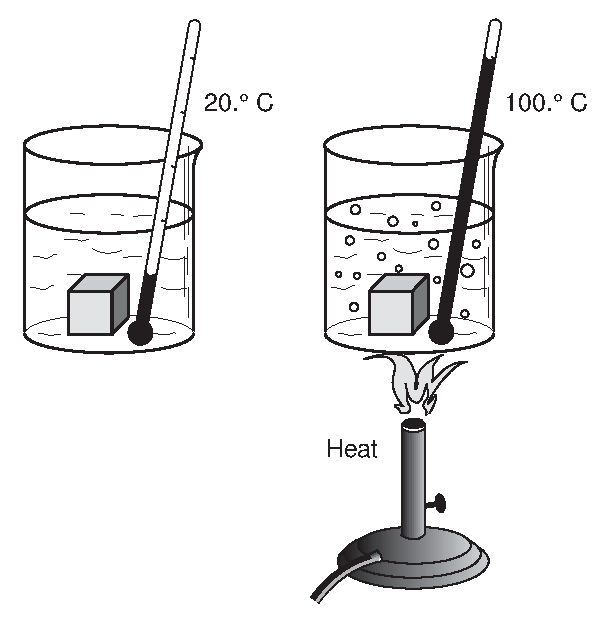
\includegraphics[keepaspectratio,scale=0.75]{Jan2002-Q66}
    \end{center}
    The maximum amount of heat absorbed by the lead cube during the experiment was approximately:
    \begin{multicols}{2}
    \begin{choices}
      \correctchoice{\SI{0.31}{\kilo\joule}}
        \wrongchoice{\SI{10}{\kilo\joule}}
        \wrongchoice{\SI{60}{\kilo\joule}}
        \wrongchoice{\SI{790}{\kilo\joule}}
    \end{choices}
    \end{multicols}
\end{question}
}

\element{nysed}{
\begin{question}{Jan2002-Q67}
    Absolute zero is best described as the temperature at which:
    \begin{choices}
        \wrongchoice{water freezes at standard pressure}
        \wrongchoice{water is at its triple point}
        \wrongchoice{the molecules of a substance have maximum kinetic energy}
      \correctchoice{the molecules of a substance have minimum kinetic energy}
    \end{choices}
\end{question}
}

\element{nysed}{
\begin{question}{Jan2002-Q68}
    A temperature change of \SI{20}{\degreeCelsius} is equal to a temperature change of:
    \begin{multicols}{2}
    \begin{choices}
      \correctchoice{\SI{20}{\kelvin}}
        \wrongchoice{\SI{120}{\kelvin}}
        \wrongchoice{\SI{253}{\kelvin}}
        \wrongchoice{\SI{293}{\kelvin}}
    \end{choices}
    \end{multicols}
\end{question}
}

\element{nysed}{
\begin{question}{Jan2002-Q69}
    Heat will always flow from object $A$ to object $B$ if object $B$ has a lower:
    \begin{multicols}{2}
    \begin{choices}
        \wrongchoice{mass}
        \wrongchoice{total energy}
      \correctchoice{temperature}
        \wrongchoice{specific heat}
    \end{choices}
    \end{multicols}
\end{question}
}

\element{nysed}{
\begin{question}{Jan2002-Q70}
    Equal amounts of heat energy are given off by \SI{1.0}{\kilo\gram} samples of aluminum,
        iron, platinum, and zinc, all initially at \SI{100}{\degreeCelsius}.
    Which sample has the greatest decrease in temperature?
    %% TODO: add specific heats to ref.tex
    %% Specific Heats
    %% Al 0.91 kJ per kg per K
    %% Fe 0.45 kJ per kg per K
    %% Pa 0.13 kJ per kg per K
    %% Zn 0.39 kJ per kg per K
    \begin{multicols}{2}
    \begin{choices}
        \wrongchoice{aluminum}
        \wrongchoice{iron}
      \correctchoice{platinum}
        \wrongchoice{zinc}
    \end{choices}
    \end{multicols}
\end{question}
}

\element{nysed}{
\begin{question}{Jan2002-Q71}
    The graph below shows the temperature of \SI{3.0}{\kilo\gram} of a pure substance initially in the solid phase as heat is added to it at a constant rate.
    \begin{center}
    \begin{tikzpicture}
        \begin{axis}[
            axis y line=left, 
            axis x line=bottom, 
            axis line style={->},
            ylabel={temperature},
            y unit=\si{\degreeCelsius},
            ytick=\empty,
            xlabel={heat added},
            x unit=\si{\kilo\joule},
            xtick={0,75,150},
            ymin=0,ymax=400,
            xmin=0,xmax=225,
            width=0.8\columnwidth,
            height=0.5\columnwidth,
        ]
        \addplot[line width=1pt,mark=\empty] plot coordinates { (0,0) (75,200) (150,200) (225,400) };
        \draw[dashed] (axis cs:75,0) -- (axis cs:75,200);
        \draw[dashed] (axis cs:150,0) -- (axis cs:150,200);
        \end{axis}
    \end{tikzpicture}
    \end{center}
    The substance is most likely:
    \begin{multicols}{2}
    \begin{choices}
        \wrongchoice{alcohol}
        \wrongchoice{silver}
        \wrongchoice{copper}
      \correctchoice{lead}
    \end{choices}
    \end{multicols}
\end{question}
}

\element{nysed}{
\begin{question}{Jan2002-Q72}
    As a large quantity of salt is added to a container of boiling water, the water:
    \begin{choices}
        \wrongchoice{stops boiling because the boiling point decreases}
      \correctchoice{stops boiling because the boiling point increases}
        \wrongchoice{boils faster because the boiling point decreases}
        \wrongchoice{boils faster because the boiling point increases}
    \end{choices}
\end{question}
}

\element{nysed}{
\begin{question}{Jan2002-Q73}
    The total effect of all the processes that occur in the universe is an increase in:
    \begin{multicols}{2}
    \begin{choices}
      \correctchoice{entropy}
        \wrongchoice{temperature}
        \wrongchoice{order}
        \wrongchoice{energy}
    \end{choices}
    \end{multicols}
\end{question}
}

\element{nysed}{
\begin{question}{Jan2002-Q74}
    Which graph best represents the relationship between volume and absolute temperature for a fixed mass of an ideal gas at constant pressure?
    \begin{multicols}{2}
    \begin{choices}
        \AMCboxDimensions{down=-2.5em}
        \correctchoice{
            \begin{tikzpicture}
                \begin{axis}[
                    axis y line=left, 
                    axis x line=bottom, 
                    axis line style={->},
                    xlabel={temperature},
                    xtick=\empty,
                    ylabel={volume},
                    ytick=\empty,
                    xmin=0,xmax=11,
                    ymin=0,ymax=11,
                    width=\columnwidth,
                ]
                \addplot[line width=1pt,domain=0:10]{x};
                \end{axis}
            \end{tikzpicture}
        }
        \wrongchoice{
            \begin{tikzpicture}
                \begin{axis}[
                    axis y line=left, 
                    axis x line=bottom, 
                    axis line style={->},
                    xlabel={temperature},
                    xtick=\empty,
                    ylabel={volume},
                    ytick=\empty,
                    xmin=0,xmax=11,
                    ymin=0,ymax=11,
                    width=\columnwidth,
                ]
                \addplot[line width=1pt,domain=0:10]{10-x};
                \end{axis}
            \end{tikzpicture}
        }
        \wrongchoice{
            \begin{tikzpicture}
                \begin{axis}[
                    axis y line=left, 
                    axis x line=bottom, 
                    axis line style={->},
                    xlabel={temperature},
                    xtick=\empty,
                    ylabel={volume},
                    ytick=\empty,
                    xmin=0,xmax=11,
                    ymin=0,ymax=11,
                    width=\columnwidth,
                ]
                \addplot[line width=1pt,domain=0:10]{0.1*x*x};
                \end{axis}
            \end{tikzpicture}
        }
        \wrongchoice{
            \begin{tikzpicture}
                \begin{axis}[
                    axis y line=left, 
                    axis x line=bottom, 
                    axis line style={->},
                    xlabel={temperature},
                    xtick=\empty,
                    ylabel={volume},
                    ytick=\empty,
                    xmin=0,xmax=11,
                    ymin=0,ymax=11,
                    width=\columnwidth,
                ]
                \addplot[line width=1pt,domain=0:10]{10/x};
                \end{axis}
            \end{tikzpicture}
        }
    \end{choices}
    \end{multicols}
\end{question}
}

\element{nysed}{
\begin{question}{Jan2002-Q75}
    As the pressure of a fixed mass of gas is increased at constant temperature,
        the density of that gas:
    \begin{choices}
        \wrongchoice{decreases}
      \correctchoice{increases}
        \wrongchoice{remains the same}
    \end{choices}
\end{question}
}


%% Section June2001
%%--------------------
\newcommand{\myJuneZeroOneQsixtySixTikz}{
    \begin{tikzpicture}
        \begin{axis}[
            axis y line=left, 
            axis x line=bottom, 
            axis line style={->},
            ylabel={temperature},
            y unit=\si{\degreeCelsius},
            ytick={0,20,40,60,80,100,120,140,160},
            xlabel={time},
            x unit=\si{\minute},
            xtick={0,2,4,6,8,10,12,14,16,18,20,22,24},
            ymin=0,ymax=170,
            xmin=0,xmax=25.5,
            grid=major,
            width=\columnwidth,
            height=0.618\columnwidth,
        ]
        \addplot[line width=1pt,domain=0:2] {160-20*x};
        \addplot[line width=1pt,domain=2:9] {120};
        \addplot[line width=1pt,domain=9:17] {120-6.25*(x-9)};
        \addplot[line width=1pt,domain=17:20] {70};
        \addplot[line width=1pt,domain=20:25] {70-10*(x-20)};
        \end{axis}
    \end{tikzpicture}
}
\element{nysed}{
\begin{question}{June2001-Q66}
    The graph below represents a cooling curve for \SI{10}{\kilo\gram} of a substance as it cools from a vapor at \SI{160}{\degreeCelsius} to a solid at \SI{20}{\degreeCelsius}.
    Energy is removed from the sample at a constant rate.
    \begin{center}
        \myJuneZeroOneQsixtySixTikz
    \end{center}
    While the substance is cooling during the liquid phase,
        the average kinetic energy of the molecules of the substance:
    \begin{choices}
      \correctchoice{decreases}
        \wrongchoice{increases}
        \wrongchoice{remains the same}
    \end{choices}
\end{question}
}

\element{nysed}{
\begin{question}{June2001-Q67}
    The graph below represents a cooling curve for \SI{10}{\kilo\gram} of a substance as it cools from a vapor at \SI{160}{\degreeCelsius} to a solid at \SI{20}{\degreeCelsius}.
    Energy is removed from the sample at a constant rate.
    \begin{center}
        \myJuneZeroOneQsixtySixTikz
    \end{center}
    The melting point of the substance is:
    \begin{multicols}{2}
    \begin{choices}
        \wrongchoice{\SI{0}{\degreeCelsius}}
      \correctchoice{\SI{70}{\degreeCelsius}}
        \wrongchoice{\SI{100}{\degreeCelsius}}
        \wrongchoice{\SI{120}{\degreeCelsius}}
    \end{choices}
    \end{multicols}
\end{question}
}


\element{nysed}{
\begin{question}{June2001-Q68}
    What is the change in temperature of a sample of water as it is heated from its freezing point to its boiling point at standard pressure?
    \begin{multicols}{2}
    \begin{choices}
        \wrongchoice{\SI{373}{\kelvin}}
        \wrongchoice{\SI{273}{\kelvin}}
        \wrongchoice{\SI{212}{\kelvin}}
      \correctchoice{\SI{100}{\kelvin}}
    \end{choices}
    \end{multicols}
\end{question}
}

\element{nysed}{
\begin{question}{June2001-Q69}
    Equal amounts of heat are applied to equal masses of four different substances initially at \SI{-10}{\degreeCelsius}.
    Which substance has the largest change in temperature?
    %% Al    0.91 kJ per kg per K
    %% H20  4.186 kJ per kg per K
    %% ice   2.05 kJ per kg per K
    %% Fe    0.45 kJ per kg per K
    %% ethyl  2.4 kJ per kg per K
    \begin{multicols}{2}
    \begin{choices}
        \wrongchoice{aluminum}
        \wrongchoice{ice}
      \correctchoice{iron}
        \wrongchoice{alcohol}
    \end{choices}
    \end{multicols}
\end{question}
}

\element{nysed}{
\begin{question}{June2001-Q70}
    Why do some transportation agencies spread a mixture of sand and salt on icy roads in winter?
    \begin{choices}
        \wrongchoice{Sand decreases the frictional force between vehicle tires and the road, and salt lowers the melting point of ice.}
        \wrongchoice{Sand decreases the frictional force between vehicle tires and the road, and salt raises the melting point of ice.}
        \wrongchoice{Sand increases the frictional force between vehicle tires and the road, and salt raises the melting point of ice.}
      \correctchoice{Sand increases the frictional force between vehicle tires and the road, and salt lowers the melting point of ice.}
    \end{choices}
\end{question}
}

\element{nysed}{
\begin{question}{June2001-Q71}
    The air pressure inside an automobile tire is lower during cold weather than during warm weather.
    The lower air pressure is most likely due to:
    \begin{choices}
        \wrongchoice{an increase in molecular potential energy of the air molecules in the tire}
      \correctchoice{a decrease in the speed of the air molecules in the tire}
        \wrongchoice{salt on the roads producing a decrease in tire volume}
        \wrongchoice{cold air in the tire producing an increase in tire volume}
    \end{choices}
\end{question}
}

\element{nysed}{
\begin{question}{June2001-Q72}
    Which graph best represents the relationship between volume and absolute temperature for a fixed mass of an ideal gas at constant pressure?
    %% NOTE: duplicate of Jan2002-Q74
    \begin{multicols}{2}
    \begin{choices}
        \AMCboxDimensions{down=-2.5em}
        \wrongchoice{
            \begin{tikzpicture}
                \begin{axis}[
                    axis y line=left, 
                    axis x line=bottom, 
                    axis line style={->},
                    xlabel={temperature},
                    xtick=\empty,
                    ylabel={volume},
                    ytick=\empty,
                    xmin=0,xmax=11,
                    ymin=0,ymax=11,
                    width=\columnwidth,
                ]
                \addplot[line width=1pt,domain=0:10]{10/x};
                \end{axis}
            \end{tikzpicture}
        }
        \wrongchoice{
            \begin{tikzpicture}
                \begin{axis}[
                    axis y line=left, 
                    axis x line=bottom, 
                    axis line style={->},
                    xlabel={temperature},
                    xtick=\empty,
                    ylabel={volume},
                    ytick=\empty,
                    xmin=0,xmax=11,
                    ymin=0,ymax=11,
                    width=\columnwidth,
                ]
                \addplot[line width=1pt,domain=0:10]{0.1*x*x};
                \end{axis}
            \end{tikzpicture}
        }
        \wrongchoice{
            \begin{tikzpicture}
                \begin{axis}[
                    axis y line=left, 
                    axis x line=bottom, 
                    axis line style={->},
                    xlabel={temperature},
                    xtick=\empty,
                    ylabel={volume},
                    ytick=\empty,
                    xmin=0,xmax=11,
                    ymin=0,ymax=11,
                    width=\columnwidth,
                ]
                \addplot[line width=1pt,domain=0:10]{10-x};
                \end{axis}
            \end{tikzpicture}
        }
        \correctchoice{
            \begin{tikzpicture}
                \begin{axis}[
                    axis y line=left, 
                    axis x line=bottom, 
                    axis line style={->},
                    xlabel={temperature},
                    xtick=\empty,
                    ylabel={volume},
                    ytick=\empty,
                    xmin=0,xmax=11,
                    ymin=0,ymax=11,
                    width=\columnwidth,
                ]
                \addplot[line width=1pt,domain=0:10]{x};
                \end{axis}
            \end{tikzpicture}
        }
    \end{choices}
    \end{multicols}
\end{question}
}

\element{nysed}{
\begin{question}{June2001-Q73}
    Heat will flow from a region of low temperature to a region of higher temperature if:
    \begin{choices}
        \wrongchoice{the specific heat of the cooler region is greater than the specific heat of the warmer region}
        \wrongchoice{the temperature of the cooler region is near absolute zero}
      \correctchoice{work is done to produce the flow}
        \wrongchoice{the cooler region is liquid and the warmer region is solid}
    \end{choices}
\end{question}
}

\element{nysed}{
\begin{question}{June2001-Q74}
    What is the minimum heat required to change \SI{5.0}{\kilo\gram} of copper at \SI{1083}{\degreeCelsius} from a solid to a liquid?
    %% Cu meltin temp  1084 C
    %% Cu specific heat 0.39 KJ per Kg per K
    %% Cu latent heat   205 KJ per Kg
    \begin{multicols}{2}
    \begin{choices}
        \wrongchoice{\SI{0.20}{\kilo\joule}}
        \wrongchoice{\SI{0.39}{\kilo\joule}}
        \wrongchoice{\SI{41}{\kilo\joule}}
      \correctchoice{\SI{1.0e3}{\kilo\joule}}
    \end{choices}
    \end{multicols}
\end{question}
}

\element{nysed}{
\begin{question}{June2001-Q75}
    When a box of beakers was dropped, the beakers broke into many pieces.
    Dropping the box a second time could \emph{not} cause the pieces to reform into the original beakers because this would require entropy to:
    \begin{choices}
      \correctchoice{decrease}
        \wrongchoice{increase}
        \wrongchoice{remain the same}
    \end{choices}
\end{question}
}


%% Section Jan2001
%%--------------------
\newcommand{\myJanZeroOneQsixtySixTikz}{
    \begin{tikzpicture}
        \begin{axis}[
            clip=false,
            axis y line=left, 
            axis x line=bottom, 
            axis line style={->},
            ylabel={temperature},
            y unit=\si{\degreeCelsius},
            ytick={0,25,50,75,100,125,150,175,200},
            xlabel={time},
            x unit=\si{\minute},
            xtick={0,5,10,15,20,25,30,35,40},
            ymin=0,ymax=225,
            xmin=0,xmax=45,
            grid=major,
            width=\columnwidth,
            height=0.618\columnwidth,
        ]
        \addplot[line width=1pt,domain=0:5,font=\small] {25+5*x}
            node[pos=0,anchor=north west] {$A$}
            node[pos=1,anchor=south] {$B$};
        \addplot[line width=1pt,domain=5:10,font=\small] {50}
            node[pos=1,anchor=south] {$C$};
        \addplot[line width=1pt,domain=10:15,font=\small] {50 + 15*(x-10)}
            node[pos=1,anchor=south] {$D$};
        \addplot[line width=1pt,domain=15:30,font=\small] {125}
            node[pos=1,anchor=south] {$E$};
        \addplot[line width=1pt,domain=30:40,font=\small] {125 + 7.5*(x-30)}
            node[pos=1,anchor=south] {$F$};
        \end{axis}
    \end{tikzpicture}
}

\element{nysed}{
\begin{question}{Jan2001-Q66}
    The graph below represents changes in a \SI{5.00}{\kilo\gram} sample of a substance as it absorbs heat at a constant rate of \SI{41.9}{\kilo\joule\per\minute}.
    \begin{center}
        \myJanZeroOneQsixtySixTikz
    \end{center}
    %What is the minimum amount of heat absorbed
    %    by \SI{1.00}{\kilo\gram} of the substance
    %    during interval $BE$?
    Which best represents the amount of heat absorbed by \SI{1.00}{\kilo\gram} of the substance during interval $BE$?
    \begin{multicols}{2}
    \begin{choices}
        \wrongchoice{\SI{105}{\kilo\joule}}
      \correctchoice{\SI{210}{\kilo\joule}}
        \wrongchoice{\SI{419}{\kilo\joule}}
        \wrongchoice{\SI{1050}{\kilo\joule}}
    \end{choices}
    \end{multicols}
\end{question}
}

\element{nysed}{
\begin{question}{Jan2001-Q67}
    The graph below represents changes in a \SI{5.00}{\kilo\gram} sample of a substance as it absorbs heat at a constant rate of \SI{41.9}{\kilo\joule\per\minute}.
    \begin{center}
        \myJanZeroOneQsixtySixTikz
    \end{center}
    The heat of vaporization of the substance is:
    \begin{multicols}{2}
    \begin{choices}
        \wrongchoice{\SI{210}{\kilo\joule\per\kilo\gram}}
      \correctchoice{\SI{125}{\kilo\joule\per\kilo\gram}}
        \wrongchoice{\SI{12.6}{\kilo\joule\per\kilo\gram}}
        \wrongchoice{\SI{629}{\kilo\joule\per\kilo\gram}}
    \end{choices}
    \end{multicols}
\end{question}
}

\element{nysed}{
\begin{question}{Jan2001-Q68}
    The graph below represents changes in a \SI{5.00}{\kilo\gram} sample of a substance as it absorbs heat at a constant rate of \SI{41.9}{\kilo\joule\per\minute}.
    \begin{center}
        \myJanZeroOneQsixtySixTikz
    \end{center}
    The boiling points of the substance is:
    \begin{multicols}{2}
    \begin{choices}
        \wrongchoice{\SI{25}{\degreeCelsius}}
        \wrongchoice{\SI{50}{\degreeCelsius}}
      \correctchoice{\SI{125}{\degreeCelsius}}
        \wrongchoice{\SI{150}{\degreeCelsius}}
    \end{choices}
    \end{multicols}
\end{question}
}

\element{nysed}{
\begin{question}{Jan2001-Q69}
    Gas molecules at the same temperature are always assumed to have:
    \begin{choices}
        \wrongchoice{uniform velocity}
        \wrongchoice{uniform acceleration}
        \wrongchoice{straight-line motion}
      \correctchoice{random motion}
    \end{choices}
\end{question}
}

\element{nysed}{
\begin{question}{Jan2001-Q70}
    A \SI{1.0e3}{\kilo\gram} block absorbs \SI{2.4e3}{\kilo\joule} of heat as its temperature rises from \SI{710}{\degreeCelsius} to \SI{720}{\degreeCelsius}.
    What is the specific heat of the block?
    \begin{multicols}{2}
    \begin{choices}
        \wrongchoice{\SI{2.4e5}{\kilo\joule\per\kilo\gram\per\degreeCelsius}}
      \correctchoice{\SI{0.24}{\kilo\joule\per\kilo\gram\per\degreeCelsius}}
        \wrongchoice{\SI{4.2e-7}{\kilo\joule\per\kilo\gram\per\degreeCelsius}}
        \wrongchoice{\SI{4.2e-8}{\kilo\joule\per\kilo\gram\per\degreeCelsius}}
    \end{choices}
    \end{multicols}
\end{question}
}

\element{nysed}{
\begin{question}{Jan2001-Q71}
    Which property determines the direction of the exchange of internal energy between two objects?
    \begin{multicols}{2}
    \begin{choices}
      \correctchoice{temperature}
        \wrongchoice{specific heat}
        \wrongchoice{mass}
        \wrongchoice{density}
    \end{choices}
    \end{multicols}
\end{question}
}

\element{nysed}{
\begin{question}{Jan2001-Q72}
    Which two quantities are measured in the same units?
    \begin{choices}
      \correctchoice{mechanical energy and heat}
        \wrongchoice{energy and power}
        \wrongchoice{momentum and work}
        \wrongchoice{work and power}
    \end{choices}
\end{question}
}

\element{nysed}{
\begin{question}{Jan2001-Q73}
    Which graph best represents the relationship between the average molecular kinetic energy ($\overline{KE}$) of an ideal gas and its absolute temperature?
    \begin{multicols}{2}
    \begin{choices}
        \AMCboxDimensions{down=-2.5em}
        \correctchoice{
            \begin{tikzpicture}
                \begin{axis}[
                    axis y line=left, 
                    axis x line=bottom, 
                    axis line style={->},
                    xlabel={temperature},
                    xtick=\empty,
                    ylabel={$\overline{KE}$},
                    ytick=\empty,
                    xmin=0,xmax=11,
                    ymin=0,ymax=11,
                    width=\columnwidth,
                ]
                \addplot[line width=1pt,domain=0:10]{x};
                \end{axis}
            \end{tikzpicture}
        }
        \wrongchoice{
            \begin{tikzpicture}
                \begin{axis}[
                    axis y line=left, 
                    axis x line=bottom, 
                    axis line style={->},
                    xlabel={temperature},
                    xtick=\empty,
                    ylabel={$\overline{KE}$},
                    ytick=\empty,
                    xmin=0,xmax=11,
                    ymin=0,ymax=11,
                    width=\columnwidth,
                ]
                \addplot[line width=1pt,domain=0:10]{10-x};
                \end{axis}
            \end{tikzpicture}
        }
        \wrongchoice{
            \begin{tikzpicture}
                \begin{axis}[
                    axis y line=left, 
                    axis x line=bottom, 
                    axis line style={->},
                    xlabel={temperature},
                    xtick=\empty,
                    ylabel={$\overline{KE}$},
                    ytick=\empty,
                    xmin=0,xmax=11,
                    ymin=0,ymax=11,
                    width=\columnwidth,
                ]
                \addplot[line width=1pt,domain=0:10]{10 - 0.1*x*x};
                \end{axis}
            \end{tikzpicture}
        }
        \wrongchoice{
            \begin{tikzpicture}
                \begin{axis}[
                    axis y line=left, 
                    axis x line=bottom, 
                    axis line style={->},
                    xlabel={temperature},
                    xtick=\empty,
                    ylabel={$\overline{KE}$},
                    ytick=\empty,
                    xmin=0,xmax=11,
                    ymin=0,ymax=11,
                    width=\columnwidth,
                ]
                \addplot[line width=1pt,domain=0:10]{10/x};
                \end{axis}
            \end{tikzpicture}
        }
    \end{choices}
    \end{multicols}
\end{question}
}

\element{nysed}{
\begin{question}{Jan2001-Q74}
    Equal masses of zinc and copper at room temperature are placed in an oven that supplies heat energy at a rate of \SI{1}{\kilo\joule\per\minute}.
    Compared to the time needed for the zinc sample to reach its melting point,
        the time needed for the copper sample to reach its melting point will be:
    %% Zn 0.39 kJ per kg per K
    %% Cu 419 C
    %% Cu 0.39 kJ per kg per K
    %% Cu 1084 C
    \begin{choices}
        \wrongchoice{less}
      \correctchoice{greater}
        \wrongchoice{the same}
    \end{choices}
\end{question}
}

\element{nysed}{
\begin{question}{Jan2001-Q75}
    As the volume of a fixed mass of an ideal gas increases at constant temperature,
        the product of the pressure and volume of the gas:
    \begin{choices}
        \wrongchoice{decreases}
        \wrongchoice{increases}
      \correctchoice{remains the same}
    \end{choices}
\end{question}
}


%% Section June2000
%%--------------------
\element{nysed}{
\begin{question}{June2000-Q66}
    Which substance remains a liquid over the \emph{smallest} temperature range?
    %% Cu  1084   4667  range 3583
    %% Ag   879   4013  range 3132
    %% Pb  327.5  3182  range 2854.5
    %% Fe  1149   5198  range 40049
    \begin{multicols}{2}
    \begin{choices}
        \wrongchoice{copper}
        \wrongchoice{silver}
      \correctchoice{lead}
        \wrongchoice{iron}
    \end{choices}
    \end{multicols}
\end{question}
}

\element{nysed}{
\begin{question}{June2000-Q67}
    While orbiting Earth, the space shuttle has recorded temperature ranging from \SIrange{398}{118}{\kelvin}.
    These temperatures correspond to Celsius ranging from:
    \begin{choices}
        \wrongchoice{\SIrange{125}{-391}{\degreeCelsius}}
      \correctchoice{\SIrange{125}{-155}{\degreeCelsius}}
        \wrongchoice{\SIrange{671}{391}{\degreeCelsius}}
        \wrongchoice{\SIrange{671}{155}{\degreeCelsius}}
    \end{choices}
\end{question}
}

\element{nysed}{
\begin{question}{June2000-Q68}
    What is the total amount of energy needed to change the temperature of \SI{0.20}{\kilo\gram} of lead from \SI{20}{\degreeCelsius} to \SI{30}{\degreeCelsius}?
    %% Pb 0.13  kJ per kg per K
    %% Pb 327.5 K
    \begin{multicols}{2}
    \begin{choices}
      \correctchoice{\SI{0.26}{\kilo\joule}}
        \wrongchoice{\SI{0.65}{\kilo\joule}}
        \wrongchoice{\SI{0.84}{\kilo\joule}}
        \wrongchoice{\SI{1.3}{\kilo\joule}}
    \end{choices}
    \end{multicols}
\end{question}
}

\element{nysed}{
\begin{question}{June2000-Q69}
    When a solid sample was heated, its temperature increased but it did not melt.
    Which statement best describes the changes in the average kinetic and potential energies of the molecules of the sample?
    \begin{choices}
        \wrongchoice{Potential energy decreased and kinetic energy remained the same.}
        \wrongchoice{Potential energy increased and kinetic energy remained the same.}
        \wrongchoice{Kinetic energy decreased and potential energy remained the same.}
      \correctchoice{Kinetic energy increased and potential energy remained the same.}
    \end{choices}
\end{question}
}

\element{nysed}{
\begin{question}{June2000-Q70}
    How are the boiling point of water and the melting points of ice affected by a decrease in pressure?
    \begin{choices}
        \wrongchoice{The boiling point of water increases, and the melting point of ice increases}
        \wrongchoice{The boiling point of water increases, and the melting point of ice decreases}
      \correctchoice{The boiling point of water decreases, and the melting point of ice increases}
        \wrongchoice{The boiling point of water decreases, and the melting point of ice decreases}
    \end{choices}
\end{question}
}

\element{nysed}{
\begin{question}{June2000-Q71}
    A \SI{1.0}{\kilo\gram} sample of water is boiling at \SI{100}{\degreeCelsius} in an open container.
    If a \SI{0.50}{\kilo\gram} piece of lead at \SI{300}{\degreeCelsius} is placed in the boiling water, how will the temperature of the two substances be affected?
    \begin{choices}
        \wrongchoice{The temperature of the water will decrease, and the temperature of the lead will remain the same.}
        \wrongchoice{The temperature of the water will increase, and the temperature of the lead will remain the same.}
      \correctchoice{The temperature of the water will remain the same, and the temperature of the lead will decrease.}
        \wrongchoice{The temperature of the water will remain the same, and the temperature of the lead will remain the same.}
    \end{choices}
\end{question}
}

\element{nysed}{
\begin{question}{June2000-Q72}
    Which graph best represents the relationship between pressure and volume for a fixed mass of an ideal gas at constant temperature?
    \begin{multicols}{2}
    \begin{choices}
        \AMCboxDimensions{down=-2.5em}
        \correctchoice{
            \begin{tikzpicture}
                \begin{axis}[
                    axis y line=left, 
                    axis x line=bottom, 
                    axis line style={->},
                    xlabel={volume},
                    xtick=\empty,
                    ylabel={pressure},
                    ytick=\empty,
                    xmin=0,xmax=11,
                    ymin=0,ymax=11,
                    width=\columnwidth,
                ]
                \addplot[line width=1pt,domain=0:10]{10/x};
                \end{axis}
            \end{tikzpicture}
        }
        \wrongchoice{
            \begin{tikzpicture}
                \begin{axis}[
                    axis y line=left, 
                    axis x line=bottom, 
                    axis line style={->},
                    xlabel={volume},
                    xtick=\empty,
                    ylabel={pressure},
                    ytick=\empty,
                    xmin=0,xmax=11,
                    ymin=0,ymax=11,
                    width=\columnwidth,
                ]
                \addplot[line width=1pt,domain=0:10]{0.1*x*x};
                \end{axis}
            \end{tikzpicture}
        }
        \wrongchoice{
            \begin{tikzpicture}
                \begin{axis}[
                    axis y line=left, 
                    axis x line=bottom, 
                    axis line style={->},
                    xlabel={volume},
                    xtick=\empty,
                    ylabel={pressure},
                    ytick=\empty,
                    xmin=0,xmax=11,
                    ymin=0,ymax=11,
                    width=\columnwidth,
                ]
                \addplot[line width=1pt,domain=0:10]{8};
                \end{axis}
            \end{tikzpicture}
        }
        \wrongchoice{
            \begin{tikzpicture}
                \begin{axis}[
                    axis y line=left, 
                    axis x line=bottom, 
                    axis line style={->},
                    xlabel={volume},
                    xtick=\empty,
                    ylabel={pressure},
                    ytick=\empty,
                    xmin=0,xmax=11,
                    ymin=0,ymax=11,
                    width=\columnwidth,
                ]
                \addplot[line width=1pt,domain=0:10]{x};
                \end{axis}
            \end{tikzpicture}
        }
    \end{choices}
    \end{multicols}
\end{question}
}


\element{nysed}{
\begin{question}{June2000-Q73}
    A given mass of an ideal gas is enclosed in a rigid walled container.
    If the Kelvin temperature of the gas is doubled,
        its pressure will be:
    \begin{multicols}{2}
    \begin{choices}
        \wrongchoice{halved}
      \correctchoice{doubled}
        \wrongchoice{quartered}
        \wrongchoice{quadrupled}
    \end{choices}
    \end{multicols}
\end{question}
}

\element{nysed}{
\begin{question}{June2000-Q74}
    In a diesel engine, the piston compresses gases in a cylinder.
    Why does the temperature of the gases rise during this process?
    \begin{choices}
        \wrongchoice{Heat enters the cylinder from the surroundings.}
        \wrongchoice{Heat is expelled through the exhaust system.}
        \wrongchoice{Work is done on the surroundings by the gases.}
      \correctchoice{Work is done by the piston on the gases.}
    \end{choices}
\end{question}
}

\element{nysed}{
\begin{question}{June2000-Q75}
    A commercial freezer vaporized ammonia in its cooling coils to remove heat from an ice machine.
    How much ammonia at \SI{-33}{\degreeCelsius} must be vaporized to remove \SI{6 850}{\kilo\joule} of heat from the ice machine?
    %% heat of fusion 331.37 kJ/kg
    \begin{multicols}{2}
    \begin{choices}
        \wrongchoice{\SI{0.200}{\kilo\gram}}
        \wrongchoice{\SI{5.00}{\kilo\gram}}
      \correctchoice{\SI{20.6}{\kilo\gram}}
        \wrongchoice{\SI{1370}{\kilo\gram}}
    \end{choices}
    \end{multicols}
\end{question}
}


%% Section June1999
%%--------------------
\newcommand{\myJuneNineNineQsixtySixTikz}{
\begin{tikzpicture}
    \begin{axis}[
        axis y line=left, 
        axis x line=bottom, 
        axis line style={->},
        ylabel={temperature},
        y unit=\si{\degreeCelsius},
        ytick={20,40,60,80,100,120,140,160,180},
        xlabel={time},
        clip=false,
        x unit=\si{\minute},
        xtick={0,2,4,6,8,10,12},
        ymin=20,ymax=180,
        xmin=0,xmax=12,
        width=\columnwidth,
        height=0.618\columnwidth,
        grid=major,
    ]
    \addplot[line width=1pt,domain=0:2,font=\small]{20 + 25*x}
        node[pos=0,anchor=west] {$A$}
        node[pos=1,anchor=north] {$B$}
        node[pos=0.5,anchor=south,rotate=45] {solid};
    \addplot[line width=1pt,domain=2:4,font=\small]{70}
        node[pos=1,anchor=north] {$C$};
    \addplot[line width=1pt,domain=4:7,font=\small]{70 + 50*(x-4)/3}
        node[pos=1,anchor=north] {$D$}
        node[pos=0.5,anchor=south,rotate=35,font=\small] {liquid};
    \addplot[line width=1pt,domain=7:11]{120}
        node[pos=1,anchor=north] {$E$};
    \addplot[line width=1pt,domain=11:12,font=\small]{120+40*(x-11)}
        node[pos=1,anchor=south] {$F$}
        node[pos=0.5,anchor=south,rotate=50] {gas};
    \end{axis}
\end{tikzpicture}
}

\element{nysed}{
\begin{question}{June1999-Q66}
    The graph below, which represents the changes in a \SI{2.0}{\kilo\gram} sample of a substance as it absorbs heat at a constant rate of \SI{15}{\kilo\joule\per\minute}.
    \begin{center}
        \myJuneNineNineQsixtySixTikz
    \end{center}
    %% start question
    During which two intervals on the graph is the average kinetic energy of the molecules in the sample increasing?
    \begin{multicols}{2}
    \begin{choices}
      \correctchoice{$AB$ and $CD$}
        \wrongchoice{$BC$ and $DE$}
        \wrongchoice{$BC$ and $EF$}
        \wrongchoice{$DE$ and $EF$}
    \end{choices}
    \end{multicols}
\end{question}
}

\element{nysed}{
\begin{question}{June1999-Q67}
    The graph below, which represents the changes in a \SI{2.0}{\kilo\gram} sample of a substance as it absorbs heat at a constant rate of \SI{15}{\kilo\joule\per\minute}.
    \begin{center}
        \myJuneNineNineQsixtySixTikz
    \end{center}
    %% start question
    What is the specific heat of the substance in the solid phase?
    \begin{multicols}{2}
    \begin{choices}
      \correctchoice{\SI{0.21}{\kilo\joule\per\kilo\gram\per\degreeCelsius}}
        \wrongchoice{\SI{0.30}{\kilo\joule\per\kilo\gram\per\degreeCelsius}}
        \wrongchoice{\SI{0.43}{\kilo\joule\per\kilo\gram\per\degreeCelsius}}
        \wrongchoice{\SI{0.60}{\kilo\joule\per\kilo\gram\per\degreeCelsius}}
    \end{choices}
    \end{multicols}
\end{question}
}

\element{nysed}{
\begin{question}{June1999-Q68}
    What is the ratio of a temperature change of \SI{1}{\kelvin} to a temperature change of \SI{1}{\degreeCelsius}?
    \begin{multicols}{2}
    \begin{choices}
      \correctchoice{$1:1$}
        \wrongchoice{$2:1$}
        \wrongchoice{$273:1$}
        \wrongchoice{$1:273$}
    \end{choices}
    \end{multicols}
\end{question}
}

\element{nysed}{
\begin{question}{June1999-Q69}
    The amount of heat energy liberated by a sample of water depends upon its:
    \begin{choices}
        \wrongchoice{temperature change, only}
        \wrongchoice{temperature change and mass, only}
        \wrongchoice{temperature change and phase, only}
      \correctchoice{temperature change, mass, and phase}
    \end{choices}
\end{question}
}

\element{nysed}{
\begin{question}{June1999-Q70}
    Approximately how much heat is required to vaporize \SI{2.0e-3}{\kilo\gram} of tungsten at its boiling point?
    %% NOTE: provide info in question
    %% Heat of Vaporization: 824 kJ/mol 
    %% molar mass: 0.183 kg/mol
    %% Heat of Vaporization: 4502 kJ/kg
    \begin{multicols}{2}
    \begin{choices}
        \wrongchoice{\SI{0.38}{\kilo\joule}}
        \wrongchoice{\SI{4.5}{\kilo\joule}}
      \correctchoice{\SI{8.7}{\kilo\joule}}
        \wrongchoice{\SI{11}{\kilo\joule}}
    \end{choices}
    \end{multicols}
\end{question}
}

\element{nysed}{
\begin{question}{June1999-Q71}
    The temperature at which no thermal energy can be transferred from object to another is:
    \begin{multicols}{2}
    \begin{choices}
        \wrongchoice{\SI{-273}{\kelvin}}
      \correctchoice{\SI{0}{\kelvin}}
        \wrongchoice{\SI{0}{\degreeCelsius}}
        \wrongchoice{\SI{273}{\degreeCelsius}}
    \end{choices}
    \end{multicols}
\end{question}
}

\element{nysed}{
\begin{question}{June1999-Q72}
    A covered Styrofoam cup contains \SI{0.30}{\kilo\gram} of water at \SI{100}{\degreeCelsius}.
    If \SI{0.10}{\kilo\gram} of water at \SI{20}{\degreeCelsius} is added to the Styrofoam cup,
        the temperature of the mixture will be:
    \begin{multicols}{2}
    \begin{choices}
        \wrongchoice{\SI{40}{\degreeCelsius}}
        \wrongchoice{\SI{60}{\degreeCelsius}}
      \correctchoice{\SI{80}{\degreeCelsius}}
        \wrongchoice{\SI{100}{\degreeCelsius}}
    \end{choices}
    \end{multicols}
\end{question}
}

\element{nysed}{
\begin{question}{June1999-Q73}
    A pot of water is boiling.
    When a cook throws salt into the water,
        it stops boiling because the salt:
    \begin{choices}
        \wrongchoice{lowers the water's specific heat}
        \wrongchoice{raises the water's specific heat}
        \wrongchoice{lowers the water's boiling point}
      \correctchoice{raises the water's boiling point}
    \end{choices}
\end{question}
}

\element{nysed}{
\begin{question}{June1999-Q74}
    What do the laws of thermodynamics indicate about the energy and entropy of the universe?
    \begin{choices}
        \wrongchoice{Energy is decreasing and entropy is increasing.}
        \wrongchoice{Energy is increasing and entropy is decreasing.}
        \wrongchoice{Energy is constant and entropy is decreasing.}
      \correctchoice{Energy is constant and entropy is increasing.}
    \end{choices}
\end{question}
}

\element{nysed}{
\begin{question}{June1999-Q75}
    Friction between a moving automobile's tires and the pavement causes air inside the tires to heat up.
    As the temperature of this air increases,
        the pressure in the tires:
    \begin{choices}
        \wrongchoice{decreases}
      \correctchoice{increases}
        \wrongchoice{remains the same}
    \end{choices}
\end{question}
}


%% Section June1998
%%--------------------
\element{nysed}{
\begin{question}{June1998-Q66}
    Which graph best represents the relationship between the average molecular kinetic energy ($\overline{KE}$) of an ideal gas and its absolute temperature?
    \begin{multicols}{2}
    \begin{choices}
        %% NOTE: near duplicate of Jan2001-Q73
        \AMCboxDimensions{down=-2.5em}
        \wrongchoice{
            \begin{tikzpicture}
                \begin{axis}[
                    axis y line=left, 
                    axis x line=bottom, 
                    axis line style={->},
                    xlabel={temperature},
                    xtick=\empty,
                    ylabel={$\overline{KE}$},
                    ytick=\empty,
                    xmin=0,xmax=11,
                    ymin=0,ymax=11,
                    width=\columnwidth,
                ]
                \addplot[line width=1pt,domain=0:10]{10 - 0.1*x*x};
                \end{axis}
            \end{tikzpicture}
        }
        \correctchoice{
            \begin{tikzpicture}
                \begin{axis}[
                    axis y line=left, 
                    axis x line=bottom, 
                    axis line style={->},
                    xlabel={temperature},
                    xtick=\empty,
                    ylabel={$\overline{KE}$},
                    ytick=\empty,
                    xmin=0,xmax=11,
                    ymin=0,ymax=11,
                    width=\columnwidth,
                ]
                \addplot[line width=1pt,domain=0:10]{x};
                \end{axis}
            \end{tikzpicture}
        }
        \wrongchoice{
            \begin{tikzpicture}
                \begin{axis}[
                    axis y line=left, 
                    axis x line=bottom, 
                    axis line style={->},
                    xlabel={temperature},
                    xtick=\empty,
                    ylabel={$\overline{KE}$},
                    ytick=\empty,
                    xmin=0,xmax=11,
                    ymin=0,ymax=11,
                    width=\columnwidth,
                ]
                \addplot[line width=1pt,domain=0:10]{10/x};
                \end{axis}
            \end{tikzpicture}
        }
        \wrongchoice{
            \begin{tikzpicture}
                \begin{axis}[
                    axis y line=left, 
                    axis x line=bottom, 
                    axis line style={->},
                    xlabel={temperature},
                    xtick=\empty,
                    ylabel={$\overline{KE}$},
                    ytick=\empty,
                    xmin=0,xmax=11,
                    ymin=0,ymax=11,
                    width=\columnwidth,
                ]
                \addplot[line width=1pt,domain=0:10]{8};
                \end{axis}
            \end{tikzpicture}
        }
    \end{choices}
    \end{multicols}
\end{question}
}

\element{nysed}{
\begin{question}{June1998-Q67}
    Normal human body temperature is \SI{37}{\degreeCelsius}.
    This temperature is equivalent to:
    \begin{multicols}{2}
    \begin{choices}
        \wrongchoice{\SI{63}{\kelvin}}
        \wrongchoice{\SI{137}{\kelvin}}
        \wrongchoice{\SI{236}{\kelvin}}
      \correctchoice{\SI{310}{\kelvin}}
    \end{choices}
    \end{multicols}
\end{question}
}

\element{nysed}{
\begin{question}{June1998-Q68}
    If only respective temperatures of two objects are known,
        what additional information can be determined?
    \begin{choices}
        \wrongchoice{how much heat the objects contain}
        \wrongchoice{how much heat the warmer object can supply to the colder object}
      \correctchoice{whether a heat exchange would take place if the objects were in contact}
        \wrongchoice{the total amount of energy the objects contain}
    \end{choices}
\end{question}
}

\element{nysed}{
\begin{question}{June1998-Q69}
    Equal masses of platinum, iron, aluminum, and copper are at their respective boiling points.
    Which of these metals requires the greatest amount of heat to change from liquid to the gaseous phase?
    %% Pt 22.2 kJ per kg
    %% Fe 247  kJ per kg
    %% Al 397  kJ per kg
    %% Zn 112  kJ per kg
    \begin{multicols}{2}
    \begin{choices}
      \correctchoice{aluminum}
        \wrongchoice{iron}
        \wrongchoice{platinum}
        \wrongchoice{copper}
    \end{choices}
    \end{multicols}
\end{question}
}

\element{nysed}{
\begin{question}{June1998-Q70}
    A mixture of ice and water is heated at a constant rate.
    Which graph best represents the relationship between the temperature of the mixture ($T$) and the heat added ($Q$)?
    \begin{multicols}{2}
    \begin{choices}
        \AMCboxDimensions{down=-2.5em}
        \wrongchoice{
            \begin{tikzpicture}
                \begin{axis}[
                    axis y line=left, 
                    axis x line=bottom, 
                    axis line style={->},
                    xlabel={$Q$},
                    x label style={
                        at={(current axis.right of origin)},
                        anchor=north west,
                    },
                    xtick=\empty,
                    ylabel={$T$},
                    y unit=\si{\degreeCelsius},
                    y label style={
                        at={(current axis.above origin)},
                        anchor=south east,
                    },
                    ytick={0},
                    xmin=0,xmax=11,
                    ymin=-2,ymax=11,
                    width=\columnwidth,
                ]
                \addplot[line width=1pt,domain=0:8]{0.156*x*x};
                \addplot[mark=\empty,line width=1pt] plot coordinates { (8,10) (10,10) };
                \end{axis}
            \end{tikzpicture}
        }
        \wrongchoice{
            \begin{tikzpicture}
                \begin{axis}[
                    axis y line=left, 
                    axis x line=bottom, 
                    axis line style={->},
                    xlabel={$Q$},
                    x label style={
                        at={(current axis.right of origin)},
                        anchor=north west,
                    },
                    xtick=\empty,
                    ylabel={$T$},
                    y unit=\si{\degreeCelsius},
                    y label style={
                        at={(current axis.above origin)},
                        anchor=south east,
                    },
                    ytick={0},
                    xmin=0,xmax=11,
                    ymin=-2,ymax=11,
                    width=\columnwidth,
                ]
                \addplot[mark=\empty,line width=1pt] plot coordinates { (0,0) (10,10) };
                \end{axis}
            \end{tikzpicture}
        }
        \correctchoice{
            \begin{tikzpicture}
                \begin{axis}[
                    axis y line=left, 
                    axis x line=bottom, 
                    axis line style={->},
                    xlabel={$Q$},
                    x label style={
                        at={(current axis.right of origin)},
                        anchor=north west,
                    },
                    xtick=\empty,
                    ylabel={$T$},
                    y unit=\si{\degreeCelsius},
                    y label style={
                        at={(current axis.above origin)},
                        anchor=south east,
                    },
                    ytick={0},
                    xmin=0,xmax=11,
                    ymin=-2,ymax=11,
                    width=\columnwidth,
                ]
                \addplot[mark=\empty,line width=1pt] plot coordinates { (0,0) (2,0) (8,10) (10,10) };
                \end{axis}
            \end{tikzpicture}
        }
        \wrongchoice{
            \begin{tikzpicture}
                \begin{axis}[
                    axis y line=left, 
                    axis x line=bottom, 
                    axis line style={->},
                    xlabel={$Q$},
                    x label style={
                        at={(current axis.right of origin)},
                        anchor=north west,
                    },
                    xtick=\empty,
                    ylabel={$T$},
                    y unit=\si{\degreeCelsius},
                    y label style={
                        at={(current axis.above origin)},
                        anchor=south east,
                    },
                    ytick={0},
                    xmin=0,xmax=11,
                    ymin=-2,ymax=11,
                    width=\columnwidth,
                ]
                \addplot[line width=1pt,domain=0:10] { 0.1*x*x };
                \end{axis}
            \end{tikzpicture}
        }
    \end{choices}
    \end{multicols}
\end{question}
}

\element{nysed}{
\begin{question}{June1998-Q71}
    A \SI{0.060}{\kilo\gram} ice cube at \SI{0.0}{\degreeCelsius} is placed in a glass containing \SI{0.250}{\kilo\gram} of water at \SI{25}{\degreeCelsius}.
    Which statement describes this system when equilibrium is reached? 
    [Assume no external exchange of heat.]
    \begin{choices}
      \correctchoice{The ice is completely melted and the water temperature is above \SI{0}{\degreeCelsius}}
        \wrongchoice{The ice is completely melted and the water temperature is \SI{0}{\degreeCelsius}}
        \wrongchoice{Part of the ice remains frozen and the water temperature is above \SI{0}{\degreeCelsius}}
        \wrongchoice{Part of the ice remains frozen and the water temperature is \SI{0}{\degreeCelsius}}
    \end{choices}
\end{question}
}

\element{nysed}{
\begin{question}{June1998-Q72}
    As \SI{6.00}{\kilo\gram} of liquid substance at its freezing point completely freezes,
        it gives off enough heat to melt \SI{3.00}{\kilo\gram} of ice at \SI{0}{\degreeCelsius}.
    The heat of fusion of the substance is:
    %% Enthalpy of fusion = 334 J/g
    %% Specific heat = 4.186 J/g/K
    \begin{multicols}{2}
    \begin{choices}
        \wrongchoice{\SI{2.05}{\kilo\joule\per\kilo\gram}}
        \wrongchoice{\SI{4.19}{\kilo\joule\per\kilo\gram}}
      \correctchoice{\SI{167}{\kilo\joule\per\kilo\gram}}
        \wrongchoice{\SI{668}{\kilo\joule\per\kilo\gram}}
    \end{choices}
    \end{multicols}
\end{question}
}

\element{nysed}{
\begin{question}{June1998-Q73}
    As lead melts, there is a change in its:
    \begin{choices}
        \wrongchoice{temperature}
        \wrongchoice{heat of fusion}
      \correctchoice{average molecular kinetic energy}
        \wrongchoice{average molecular kinetic energy}
    \end{choices}
\end{question}
}

\element{nysed}{
\begin{question}{June1998-Q74}
    How do the freezing point and boiling point of ocean water compare to those of distilled water?
    \begin{choices}
        \wrongchoice{Ocean water freezes at a lower temperature and boils at a lower temperature.}
      \correctchoice{Ocean water freezes at a lower temperature and boils at a higher temperature.}
        \wrongchoice{Ocean water freezes at a higher temperature and boils at a lower temperature.}
        \wrongchoice{Ocean water freezes at a higher temperature and boils at a higher temperature.}
    \end{choices}
\end{question}
}

\element{nysed}{
\begin{question}{June1998-Q75}
    A cylinder fitted with a piston contains a fixed mass of an ideal gas.
    Heat is added to the gas, causing it to expand and raise the piston.
    If all the added heat is converted to work done in raising the piston,
        the internal energy of the gas will:
    \begin{choices}
        \wrongchoice{decrease}
        \wrongchoice{increase}
      \correctchoice{remain the same}
    \end{choices}
\end{question}
}


%% Section June1997
%%--------------------
\element{nysed}{
\begin{question}{June1997-Q66}
    What is the boiling point of water at standard pressure on the Kelvin scale?
    \begin{multicols}{2}
    \begin{choices}
        \wrongchoice{\SI{100}{\kelvin}}
        \wrongchoice{\SI{212}{\kelvin}}
        \wrongchoice{\SI{273}{\kelvin}}
      \correctchoice{\SI{373}{\kelvin}}
    \end{choices}
    \end{multicols}
\end{question}
}

\element{nysed}{
\begin{question}{June1997-Q67}
    Two solid metal blocks are placed in an insulated container.
    If there is a net flow of heat between the blocks,
        they must have different:
    \begin{choices}
      \correctchoice{initial temperatures}
        \wrongchoice{melting points}
        \wrongchoice{specific heats}
        \wrongchoice{heats of fusion}
    \end{choices}
\end{question}
}

\element{nysed}{
\begin{question}{June1997-Q68}
    Samples of lead, platinum, silver and tungsten each have a mass of \SI{1.0}{\kilo\gram} and an initial temperature of \SI{20}{\degreeCelsius}.
    If \SI{10}{\kilo\joule} of heat is added to each sample,
        which sample will experience the smallest increase in temperature?
    %% NOTE: do not need specific heat values because of wording
    \begin{choices}
        \wrongchoice{lead, because it has the lowest heat of fusion}
        \wrongchoice{platinum, because it has the lowest heat of vaporization}
      \correctchoice{silver, because it has the highest specific heat}
        \wrongchoice{tungsten, because it has the highest melting point}
    \end{choices}
\end{question}
}

\element{nysed}{
\begin{question}{June1997-Q69}
    When Julianne drinks cold water,
        her body warms the water until thermal equilibrium is reached.
    If she drinks \num{6} glasses (\SI{2.5}{\kilo\gram}) of water at \SI{0}{\degreeCelsius} in a day,
        approximately how much energy must her body expend to raise the temperature of this water to her body's temperature of \SI{37}{\degreeCelsius}?
    %% Q = mc \delta T
    %% c_water = 4186 J / kg
    \begin{multicols}{2}
    \begin{choices}
        \wrongchoice{\SI{190}{\kilo\joule}}
      \correctchoice{\SI{390}{\kilo\joule}}
        \wrongchoice{\SI{840}{\kilo\joule}}
        \wrongchoice{\SI{2300}{\kilo\joule}}
    \end{choices}
    \end{multicols}
\end{question}
}

\element{nysed}{
\begin{question}{June1997-Q70}
    Which statement is consistent with the kinetic theory of ideal gases?
    \begin{choices}
        \wrongchoice{Molecules are always stationary}
        \wrongchoice{The force of attraction between molecules is large}
      \correctchoice{Molecules transfer energy through collisions}
        \wrongchoice{The size of molecules is large compared to the distance that separates them.}
    \end{choices}
\end{question}
}

\element{nysed}{
\begin{question}{June1997-Q71}
    The graph below shows temperature versus time for \SI{1.0}{\kilo\gram} of unknown material as heat is added at a constant rate.
    \begin{center}
    \begin{tikzpicture}
        \begin{axis}[
            axis y line=left, 
            axis x line=bottom, 
            axis line style={->},
            ylabel={temperature},
            ytick=\empty,
            xlabel={time},
            xtick=\empty,
            ymin=0,ymax=100,
            xmin=0,xmax=100,
            width=\columnwidth,
            height=0.618\columnwidth,
        ]
        \addplot[line width=1pt,domain=0:20]{2*x};
        \addplot[line width=1pt,domain=20:40]{40};
        \addplot[line width=1pt,domain=40:60]{40+2*(x-40)};
        \addplot[line width=1pt,domain=60:80]{80}
            node[pos=0,anchor=south] {$x$}
            node[pos=1,anchor=south] {$y$};
        \addplot[line width=1pt,domain=80:100]{80+(x-80)};
        \end{axis}
    \end{tikzpicture}
    \end{center}
    During interval $xy$, the material experiences:
    \begin{choices}
        \wrongchoice{a decrease in internal energy and a phase change}
      \correctchoice{an increase in internal energy and a phase change}
        \wrongchoice{no change in internal energy and a phase change}
        \wrongchoice{no change in internal energy and no phase change}
    \end{choices}
\end{question}
}

\element{nysed}{
\begin{question}{June1997-Q72}
    Which graph best represents the relationship between volume and absolute temperature for a fixed mass of an ideal gas at constant pressure?
    \begin{multicols}{2}
    \begin{choices}
        \AMCboxDimensions{down=-2.5em}
        \correctchoice{
            \begin{tikzpicture}
                \begin{axis}[
                    axis y line=left, 
                    axis x line=bottom, 
                    axis line style={->},
                    xlabel={temperature},
                    xtick=\empty,
                    ylabel={volume},
                    ytick=\empty,
                    xmin=0,xmax=11,
                    ymin=0,ymax=11,
                    width=\columnwidth,
                ]
                \addplot[line width=1pt,domain=0:10]{x};
                \end{axis}
            \end{tikzpicture}
        }
        \wrongchoice{
            \begin{tikzpicture}
                \begin{axis}[
                    axis y line=left, 
                    axis x line=bottom, 
                    axis line style={->},
                    xlabel={temperature},
                    xtick=\empty,
                    ylabel={volume},
                    ytick=\empty,
                    xmin=0,xmax=11,
                    ymin=0,ymax=11,
                    width=\columnwidth,
                ]
                \addplot[line width=1pt,domain=0:10]{10-x};
                \end{axis}
            \end{tikzpicture}
        }
        \wrongchoice{
            \begin{tikzpicture}
                \begin{axis}[
                    axis y line=left, 
                    axis x line=bottom, 
                    axis line style={->},
                    xlabel={temperature},
                    xtick=\empty,
                    ylabel={volume},
                    ytick=\empty,
                    xmin=0,xmax=11,
                    ymin=0,ymax=11,
                    width=\columnwidth,
                ]
                \addplot[line width=1pt,domain=0:10]{8};
                \end{axis}
            \end{tikzpicture}
        }
        \wrongchoice{
            \begin{tikzpicture}
                \begin{axis}[
                    axis y line=left, 
                    axis x line=bottom, 
                    axis line style={->},
                    xlabel={temperature},
                    xtick=\empty,
                    ylabel={volume},
                    ytick=\empty,
                    xmin=0,xmax=11,
                    ymin=0,ymax=11,
                    width=\columnwidth,
                ]
                \addplot[line width=1pt,domain=0:10]{10/x};
                \end{axis}
            \end{tikzpicture}
        }
    \end{choices}
    \end{multicols}
\end{question}
}

\element{nysed}{
\begin{question}{June1997-Q73}
    How much heat must be removed from \SI{0.50}{\kilo\gram} of mercury at \SI{-39}{\degreeCelsius} to change it from liquid to a solid?
    %% Hg -38.86 C
    %% Hg 11.3 kJ per kg
    \begin{multicols}{2}
    \begin{choices}
        \wrongchoice{\SI{1.1}{\kilo\joule}}
      \correctchoice{\SI{5.6}{\kilo\joule}}
        \wrongchoice{\SI{150}{\kilo\joule}}
        \wrongchoice{\SI{180}{\kilo\joule}}
    \end{choices}
    \end{multicols}
\end{question}
}

\element{nysed}{
\begin{question}{June1997-Q74}
    Which phase change represents a decrease in entropy?
    \begin{multicols}{2}
    \begin{choices}
        \wrongchoice{solid to gas}
        \wrongchoice{solid to liquid}
      \correctchoice{gas to liquid}
        \wrongchoice{liquid to gas}
    \end{choices}
    \end{multicols}
\end{question}
}

\element{nysed}{
\begin{question}{June1997-Q75}
    In an operating automobile,
        the pressure of the coolant in the radiator is greater than \num{1.0} atmosphere and its temperature is above \SI{100}{\degreeCelsius}.
    If the radiator's pressure cap is removed,
        the pressure of the coolant is lowered to \num{1.0} atmospheres,
        causing the boiling point of the coolant to:
    \begin{choices}
      \correctchoice{decrease}
        \wrongchoice{increase}
        \wrongchoice{remain the same}
    \end{choices}
\end{question}
}


%% Section June1996
%%--------------------
\element{nysed}{
\begin{question}{June1996-Q66}
    If the temperature of \SI{1}{\liter} of an ideal gas is increased from \SI{4}{\kelvin} to \SI{16}{\kelvin},
        the average kinetic energy of the molecules of the gas will be:
    \begin{choices}
        \wrongchoice{half as great}
        \wrongchoice{twice as great}
        \wrongchoice{one-fourth as great}
      \correctchoice{four times as great}
    \end{choices}
\end{question}
}

\newcommand{\myJuneNineSixQsixtySevenTikz}{
    \begin{tikzpicture}
        \begin{axis}[
            axis y line=left, 
            axis x line=bottom, 
            axis line style={->},
            clip=false,
            ylabel={Temperature},
            y unit=\si{\degreeCelsius},
            ytick={100,200,300,400,500},
            ymin=100,ymax=500,
            xlabel={Heat added to substance},
            x unit=\si{\kilo\joule},
            xtick={0,40,80,120,160,200},
            xmin=0,xmax=200,
            grid=major,
            width=\columnwidth,
            height=0.618\columnwidth,
        ]
        \addplot[line width=1pt,domain=0:40]{100+2.5*x}
            node[pos=0.5,anchor=south,rotate=35] {solid};
        \addplot[line width=1pt,domain=40:80]{200};
        \addplot[line width=1pt,domain=80:120]{200+5*(x-80)}
            node[pos=0.5,anchor=south,rotate=54] {liquid};
        \addplot[line width=1pt,domain=120:160]{400};
        \addplot[line width=1pt,domain=160:200]{400+2.5*(x-160)}
            node[pos=0.5,anchor=south,rotate=35] {gas};
        \end{axis}
    \end{tikzpicture}
}

\element{nysed}{
\begin{question}{June1996-Q67}
    The graph below shows the relationship between the temperature of \SI{1.0}{\kilo\gram} of pure substance and the heat energy added to the substance.
    \begin{center}
        \myJuneNineSixQsixtySevenTikz
    \end{center}
    What is the heat of fusion of the substance?
    \begin{multicols}{2}
    \begin{choices}
      \correctchoice{\SI{40}{\kilo\joule\per\kilo\gram}}
        \wrongchoice{\SI{80}{\kilo\joule\per\kilo\gram}}
        \wrongchoice{\SI{120}{\kilo\joule\per\kilo\gram}}
        \wrongchoice{\SI{160}{\kilo\joule\per\kilo\gram}}
    \end{choices}
    \end{multicols}
\end{question}
}

\element{nysed}{
\begin{question}{June1996-Q68}
    The graph below shows the relationship between the temperature of \SI{1.0}{\kilo\gram} of pure substance and the heat energy added to the substance.
    \begin{center}
        \myJuneNineSixQsixtySevenTikz
    \end{center}
    The freezing point of the substance is?
    \begin{multicols}{2}
    \begin{choices}
        \wrongchoice{\SI{400}{\degreeCelsius}}
        \wrongchoice{\SI{300}{\degreeCelsius}}
      \correctchoice{\SI{200}{\degreeCelsius}}
        \wrongchoice{\SI{100}{\degreeCelsius}}
    \end{choices}
    \end{multicols}
\end{question}
}

\element{nysed}{
\begin{question}{June1996-Q69}
    The graph below shows the relationship between the temperature of \SI{1.0}{\kilo\gram} of pure substance and the heat energy added to the substance.
    \begin{center}
        \myJuneNineSixQsixtySevenTikz
    \end{center}
    What is the specific heat of the substance as a gas?
    \begin{multicols}{2}
    \begin{choices}
      \correctchoice{\SI{0.4}{\kilo\joule\per\kilo\gram\per\degreeCelsius}}
        \wrongchoice{\SI{0.04}{\kilo\joule\per\kilo\gram\per\degreeCelsius}}
        \wrongchoice{\SI{40}{\kilo\joule\per\kilo\gram\per\degreeCelsius}}
        \wrongchoice{\SI{4}{\kilo\joule\per\kilo\gram\per\degreeCelsius}}
    \end{choices}
    \end{multicols}
\end{question}
}

\element{nysed}{
\begin{question}{June1996-Q70}
    The graph below shows the relationship between the temperature of \SI{1.0}{\kilo\gram} of pure substance and the heat energy added to the substance.
    \begin{center}
        \myJuneNineSixQsixtySevenTikz
    \end{center}
    If the initial temperature is \SI{100}{\degreeCelsius},
        the total amount of heat required to convert all of the substance to a gas is:
    \begin{multicols}{2}
    \begin{choices}
        \wrongchoice{\SI{40}{\kilo\joule}}
        \wrongchoice{\SI{80}{\kilo\joule}}
        \wrongchoice{\SI{120}{\kilo\joule}}
      \correctchoice{\SI{160}{\kilo\joule}}
    \end{choices}
    \end{multicols}
\end{question}
}

\element{nysed}{
\begin{question}{June1996-Q71}
    When a car is driven over snow,
        the snow under the tires may melt because the:
    \begin{choices}
      \correctchoice{pressure of the tires lowers the melting point of the snow}
        \wrongchoice{pressure of the tires raises the melting point of the snow}
        \wrongchoice{snow loses heat energy to the tires}
        \wrongchoice{specific heat of the snow is decreased}
    \end{choices}
\end{question}
}

\element{nysed}{
\begin{question}{June1996-Q72}
    The temperature of a water sample increased \SI{5}{\degreeCelsius} from its freezing point.
    The sample's rise in temperature on the Kelvin scale was:
    \begin{multicols}{2}
    \begin{choices}
      \correctchoice{\SI{5}{\kelvin}}
        \wrongchoice{\SI{9}{\kelvin}}
        \wrongchoice{\SI{278}{\kelvin}}
        \wrongchoice{\SI{378}{\kelvin}}
    \end{choices}
    \end{multicols}
\end{question}
}

\element{nysed}{
\begin{question}{June1996-Q73}
    Which graph best represents the relationship between pressure and absolute temperature for a fixed mass of an ideal gas in a rigid container?
    \begin{multicols}{2}
    \begin{choices}
        \AMCboxDimensions{down=-2.5em}
        \correctchoice{
            \begin{tikzpicture}
                \begin{axis}[
                    axis y line=left, 
                    axis x line=bottom, 
                    axis line style={->},
                    xlabel={temperature},
                    xtick=\empty,
                    ylabel={pressure},
                    ytick=\empty,
                    xmin=0,xmax=11,
                    ymin=0,ymax=11,
                    width=\columnwidth,
                ]
                \addplot[line width=1pt,domain=0:10]{x};
                \end{axis}
            \end{tikzpicture}
        }
        \wrongchoice{
            \begin{tikzpicture}
                \begin{axis}[
                    axis y line=left, 
                    axis x line=bottom, 
                    axis line style={->},
                    xlabel={temperature},
                    xtick=\empty,
                    ylabel={pressure},
                    ytick=\empty,
                    xmin=0,xmax=11,
                    ymin=0,ymax=11,
                    width=\columnwidth,
                ]
                \addplot[line width=1pt,domain=0:10]{0.1*x*x};
                \end{axis}
            \end{tikzpicture}
        }
        \wrongchoice{
            \begin{tikzpicture}
                \begin{axis}[
                    axis y line=left, 
                    axis x line=bottom, 
                    axis line style={->},
                    xlabel={temperature},
                    xtick=\empty,
                    ylabel={pressure},
                    ytick=\empty,
                    xmin=0,xmax=11,
                    ymin=0,ymax=11,
                    width=\columnwidth,
                ]
                \addplot[line width=1pt,domain=0:10]{10/x};
                \end{axis}
            \end{tikzpicture}
        }
        \wrongchoice{
            \begin{tikzpicture}
                \begin{axis}[
                    axis y line=left, 
                    axis x line=bottom, 
                    axis line style={->},
                    xlabel={temperature},
                    xtick=\empty,
                    ylabel={pressure},
                    ytick=\empty,
                    xmin=0,xmax=11,
                    ymin=0,ymax=11,
                    width=\columnwidth,
                ]
                \addplot[line width=1pt,domain=0:10]{10-x};
                \end{axis}
            \end{tikzpicture}
        }
    \end{choices}
    \end{multicols}
\end{question}
}

\element{nysed}{
\begin{question}{June1996-Q74}
    Which characteristic of a gas sample results from the collision of gas molecules with the walls of its container?
    \begin{choices}
        \wrongchoice{specific heat}
        \wrongchoice{condensation point}
        \wrongchoice{temperature}
      \correctchoice{pressure}
    \end{choices}
\end{question}
}

\element{nysed}{
\begin{question}{June1996-Q75}
    As the absolute temperature of a fixed mass of an ideal gas is increased at constant pressure,
        the volume occupied by the gas:
    \begin{choices}
        \wrongchoice{decreases}
      \correctchoice{increases}
        \wrongchoice{remains the same}
    \end{choices}
\end{question}
}


%% Section June1995
%%--------------------
\element{nysed}{
\begin{question}{June1995-Q66}
    Absolute zero represents a substance's minimum:
    \begin{choices}
      \correctchoice{internal molecular energy}
        \wrongchoice{gravitational potential energy}
        \wrongchoice{specific heat}
        \wrongchoice{heat of fusion}
    \end{choices}
\end{question}
}

\element{nysed}{
\begin{question}{June1995-Q67}
    At \SI{1.0}{\atm} of pressure, which substance is a solid at \SI{-51}{\degreeCelsius} and a liquid at \SI{-33}{\degreeCelsius}?
    \begin{multicols}{2}
    \begin{choices}
        \wrongchoice{ammonia}
        \wrongchoice{ethyl alcohol}
      \correctchoice{mercury}
        \wrongchoice{lead}
    \end{choices}
    \end{multicols}
\end{question}
}

\element{nysed}{
\begin{question}{June1995-Q68}
    Equal masses of four different solids, $A$, $B$, $C$, and $D$,
        are heated at a constant rate.
    The graph below represents the temperature of each solid as a function of the heat added to the solid.
    \begin{center}
    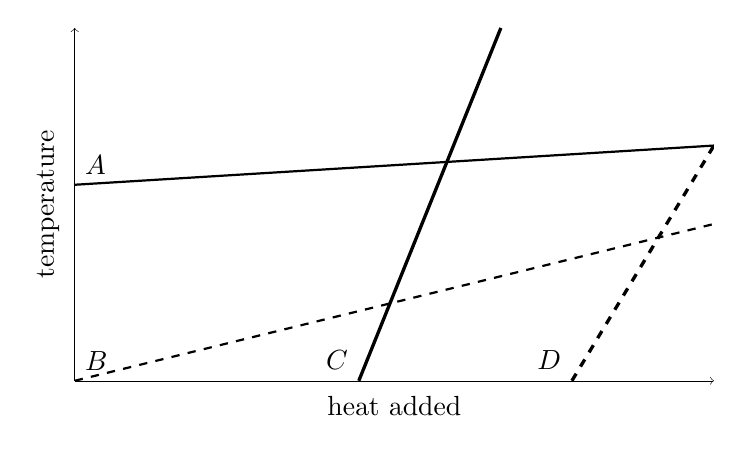
\begin{tikzpicture}
        \begin{axis}[
            axis y line=left,
            axis x line=bottom,
            axis line style={->},
            xlabel={heat added},
            xtick=\empty,
            ylabel={temperature},
            ytick=\empty,
            xmin=0,xmax=9,
            ymin=0,ymax=9,
            width=0.8\columnwidth,
            height=0.5\columnwidth,
            very thin,
        ]
        \draw[thick] (axis cs:0,5) -- (axis cs:9,6) node[pos=0,anchor=south west] {$A$};
        \draw[thick,dashed] (axis cs:0,0) -- (axis cs:9,4) node[pos=0,anchor=south west] {$B$};
        \draw[very thick] (axis cs:4,0) -- (axis cs:6,9) node[pos=0,anchor=south east] {$C$};
        \draw[very thick,dashed] (axis cs:7,0) -- (axis cs:9,6) node[pos=0,anchor=south east] {$D$};
        \end{axis}
    \end{tikzpicture}
    \end{center}
    Which solid has the greatest specific heat?
    \begin{multicols}{4}
    \begin{choices}
      \correctchoice{$A$}
        \wrongchoice{$B$}
        \wrongchoice{$C$}
        \wrongchoice{$D$}
    \end{choices}
    \end{multicols}
\end{question}
}

\element{nysed}{
\begin{question}{June1995-Q69}
    A change of \SI{10}{\degreeCelsius} is produced by adding \SI{2.4}{\kilo\joule} of heat to \SI{1.0}{\kilo\gram} of a substance.
    The substance could be:
    \begin{multicols}{2}
    \begin{choices}
      \correctchoice{silver}
        \wrongchoice{lead}
        \wrongchoice{platinum}
        \wrongchoice{aluminum}
    \end{choices}
    \end{multicols}
\end{question}
}

\element{nysed}{
\begin{question}{June1995-Q70}
    The amount of heat required to melt \SI{0.50}{\kilo\gram} of iron at its melting point is approximately:
    \begin{multicols}{2}
    \begin{choices}
        \wrongchoice{\SI{0.23}{\kilo\joule}}
        \wrongchoice{\SI{0.90}{\kilo\joule}}
        \wrongchoice{\SI{13}{\kilo\joule}}
      \correctchoice{\SI{130}{\kilo\joule}}
    \end{choices}
    \end{multicols}
\end{question}
}

\element{nysed}{
\begin{question}{June1995-Q71}
    Increasing the external pressure on a sample of water will:
    \begin{choices}
        \wrongchoice{increase its boiling point and increase its freezing point}
      \correctchoice{increase its boiling point and decrease its freezing point}
        \wrongchoice{decrease its boiling point and increase its freezing point}
        \wrongchoice{decrease its boiling point and decrease its freezing point}
    \end{choices}
\end{question}
}

\element{nysed}{
\begin{question}{June1995-Q72}
    According to the kinetic theory of gases, an ideal gas of low density has relatively large:
    \begin{choices}
        \wrongchoice{molecules}
        \wrongchoice{energy loss in molecular collisions}
        \wrongchoice{forces between molecules}
      \correctchoice{distances between molecules}
    \end{choices}
\end{question}
}

\element{nysed}{
\begin{question}{June1995-Q73}
    If the pressure on a fixed mass of an ideal gas is doubled at a constant temperature,
        the  volume of this gas sample will be:
    \begin{multicols}{2}
    \begin{choices}
        \wrongchoice{the same}
        \wrongchoice{doubled}
      \correctchoice{halved}
        \wrongchoice{quartered}
    \end{choices}
    \end{multicols}
\end{question}
}

\element{nysed}{
\begin{question}{June1995-Q74}
    According to the second law of thermodynamics,
        which phenomenon will most likely occur?
    \begin{choices}
        \wrongchoice{The entropy of the universe will steadily decrease.}
      \correctchoice{The universe will steadily become more disordered.}
        \wrongchoice{The universe will eventually reach equilibrium at absolute zero.}
        \wrongchoice{Within the universe, more heat will flow from colder to warmer regions than from warmer to colder regions.}
    \end{choices}
\end{question}
}

\element{nysed}{
\begin{question}{June1995-Q75}
    A samples of liquid ethyl alcohol is boiling.
    As more heat is added,
    the temperature of the liquid alcohol will:
    \begin{choices}
        \wrongchoice{decrease}
        \wrongchoice{increase}
      \correctchoice{remain the same}
    \end{choices}
\end{question}
}


%% Section June1994
%%--------------------
\element{nysed}{
\begin{question}{June1994-Q66}
    Which line on the graph below represents the relationship between the average kinetic energy of the molecules on an ideal gas and absolute temperature?
    \begin{center}
    \begin{tikzpicture}
        \begin{axis}[
            axis y line=left,
            axis x line=bottom,
            axis line style={->},
            xlabel={temperature},
            xtick=\empty,
            ylabel={KE\textsubscript{ave}},
            ytick=\empty,
            xmin=0,xmax=11,
            ymin=0,ymax=11,
            width=0.8\columnwidth,
            height=0.8\columnwidth,
            clip=false,
            very thin,
        ]
        \addplot[dashed,line width=1pt,mark=\empty] plot coordinates {(0,6) (4,10)} node[anchor=south east] {$A$};
        \addplot[line width=1pt,mark=\empty] plot coordinates {(0,0) (10,10)} node[anchor=south east] {$B$};
        \addplot[dotted,line width=1pt,mark=\empty] plot coordinates {(4,0) (10,6)} node[anchor=south east] {$C$};
        \addplot[line width=1pt,mark=\empty] plot coordinates {(0,4) (10,4)} node[anchor=north east] {$D$};
        \end{axis}
    \end{tikzpicture}
    \end{center}
    \begin{multicols}{4}
    \begin{choices}[o]
        \wrongchoice{$A$}
      \correctchoice{$B$}
        \wrongchoice{$C$}
        \wrongchoice{$D$}
    \end{choices}
    \end{multicols}
\end{question}
}

\element{nysed}{
\begin{question}{June1994-Q67}
    The difference between the boiling point of lead and the freezing point of lead is:
    \begin{multicols}{2}
    \begin{choices}
        \wrongchoice{\SI{328}{\kelvin}}
      \correctchoice{\SI{1412}{\kelvin}}
        \wrongchoice{\SI{1658}{\kelvin}}
        \wrongchoice{\SI{1740}{\kelvin}}
    \end{choices}
    \end{multicols}
\end{question}
}

\element{nysed}{
\begin{question}{June1994-Q68}
    Equal masses of aluminum and copper,
        both at \SI{0}{\degreeCelsius}, are placed in the same insulated can of hot water.
    Which statement describes this system at equilibrium (the net exchange of internal energy is zero)?
    \begin{choices}
        \wrongchoice{The water has a higher temperature than the aluminum and copper.}
        \wrongchoice{The aluminum has a higher temperature than the copper and water.}
        \wrongchoice{The copper has a higher temperature than the aluminum and water.}
      \correctchoice{The aluminum, copper and water have the same temperature.}
    \end{choices}
\end{question}
}

\element{nysed}{
\begin{question}{June1994-Q69}
    An unknown liquid with a mass of \SI{0.010}{\kilo\gram} absorbs \SI{0.032}{\kilo\joule} of heat.
    Its temperature rises \SI{8.0}{\degreeCelsius},
        with no change in phase.
    What is the specific heat of the unknown liquid?
    \begin{multicols}{2}
    \begin{choices}
        \wrongchoice{\SI{0.0040}{\kilo\joule\per\kilo\gram\per\degreeCelsius}}
      \correctchoice{\SI{0.40}{\kilo\joule\per\kilo\gram\per\degreeCelsius}}
        \wrongchoice{\SI{26}{\kilo\joule\per\kilo\gram\per\degreeCelsius}}
        \wrongchoice{\SI{260}{\kilo\joule\per\kilo\gram\per\degreeCelsius}}
    \end{choices}
    \end{multicols}
\end{question}
}

\element{nysed}{
\begin{question}{June1994-Q70}
    On the graph below, the four lines show the relationship between temperature and heat added to equal masses of aluminum, copper, iron and platinum in the solid phase.
    \begin{center}
    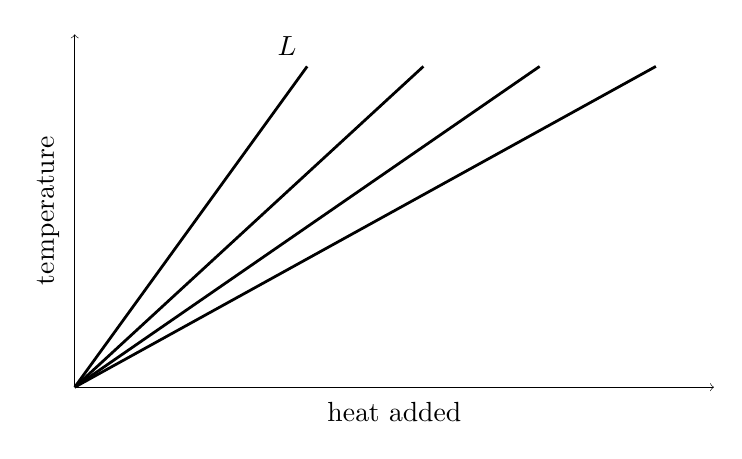
\begin{tikzpicture}
        \begin{axis}[
            axis y line=left,
            axis x line=bottom,
            axis line style={->},
            xlabel={heat added},
            xtick=\empty,
            ylabel={temperature},
            ytick=\empty,
            xmin=0,xmax=11,
            ymin=0,ymax=11,
            width=0.8\columnwidth,
            height=0.5\columnwidth,
            clip=false,
            very thin,
        ]
        \addplot[line width=1pt,mark=\empty] plot coordinates {(0,0) (4,10)} node[anchor=south east] {$L$};
        \addplot[line width=1pt,mark=\empty] plot coordinates {(0,0) (6,10)};
        \addplot[line width=1pt,mark=\empty] plot coordinates {(0,0) (8,10)};
        \addplot[line width=1pt,mark=\empty] plot coordinates {(0,0) (10,10)};
        \end{axis}
    \end{tikzpicture}
    \end{center}
    Which metal is represented by line $L$?
    \begin{multicols}{2}
    \begin{choices}
        \wrongchoice{aluminum}
        \wrongchoice{copper}
        \wrongchoice{iron}
      \correctchoice{platinum}
    \end{choices}
    \end{multicols}
\end{question}
}

\element{nysed}{
\begin{question}{June1994-Q71}
    How much heat is required to change \SI{3.0}{\kilo\gram} of ice at \SI{0.0}{\degreeCelsius} to water at \SI{0.0}{\degreeCelsius}?
    \begin{multicols}{2}
    \begin{choices}
      \correctchoice{\SI{1.0e3}{\degreeCelsius}}
        \wrongchoice{\SI{3.3e2}{\degreeCelsius}}
        \wrongchoice{\SI{2.3e3}{\degreeCelsius}}
        \wrongchoice{\SI{6.8e3}{\degreeCelsius}}
    \end{choices}
    \end{multicols}
\end{question}
}

\element{nysed}{
\begin{question}{June1994-Q72}
    According to the second law of thermodynamics,  
        as time passes, the total entropy in the universe:
    \begin{choices}
        \wrongchoice{decreases, only}
      \correctchoice{increases, only}
        \wrongchoice{remains the same}
        \wrongchoice{cyclically increases and decreases}
    \end{choices}
\end{question}
}

\element{nysed}{
\begin{question}{June1994-Q73}
    As the number of gas molecules in a rigid container at constant temperature is increased,
        the pressure on the walls of the container:
    \begin{choices}
        \wrongchoice{decreases}
      \correctchoice{increases}
        \wrongchoice{remains the same}
    \end{choices}
\end{question}
}

\element{nysed}{
\begin{question}{June1994-Q74}
    In which diagram below does the water have the highest boiling point?
    \begin{multicols}{2}
    \begin{choices}
        \AMCboxDimensions{down=-1cm}
        \wrongchoice{
            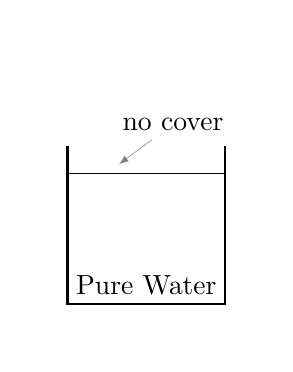
\begin{tikzpicture}
                \draw[white] (-1.5,-0.5) rectangle (1.5,3.5);
                \draw[thick] (-1,2) -- (-1,0) -- (1,0) -- (1,2);
                \draw[thin] (-1,0) rectangle (1,1.66);
                \node[anchor=south] at (0,0) {Pure Water};
                \node[pin={[pin distance=2ex,pin edge={latex-,shorten <=1pt}]80:no cover}] at (-0.5,1.66) {};
            \end{tikzpicture}
        }
        \wrongchoice{
            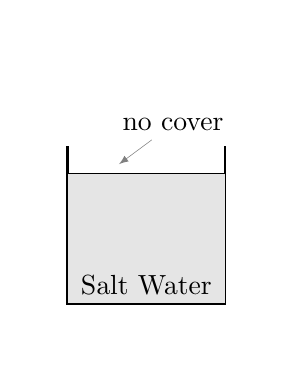
\begin{tikzpicture}
                \draw[white] (-1.5,-0.5) rectangle (1.5,3.5);
                \draw[thick] (-1,2) -- (-1,0) -- (1,0) -- (1,2);
                \draw[thin,fill=white!90!black] (-1,0) rectangle (1,1.66);
                \node[anchor=south] at (0,0) {Salt Water};
                \node[pin={[pin distance=2ex,pin edge={latex-,shorten <=1pt}]80:no cover}] at (-0.5,1.66) {};
            \end{tikzpicture}
        }
        \wrongchoice{
            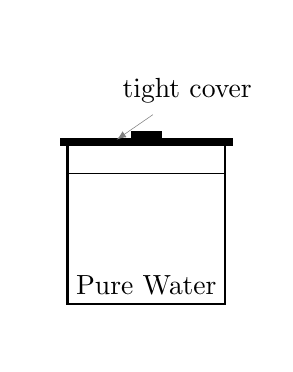
\begin{tikzpicture}
                \draw[white] (-1.5,-0.5) rectangle (1.5,3.5);
                \draw[thick] (-1,2) -- (-1,0) -- (1,0) -- (1,2);
                \draw[thin] (-1,0) rectangle (1,1.66);
                \node[anchor=south] at (0,0) {Pure Water};
                \fill (-1.1,2.0) rectangle (1.1,2.1);
                \fill (-0.2,2.1) rectangle (0.2,2.2);
                \node[pin={[pin distance=2ex,pin edge={latex-,shorten >=1pt}]80:tight cover}] at (-0.5,2.0) {};
            \end{tikzpicture}
        }
        %% ANS is 4
        \correctchoice{
            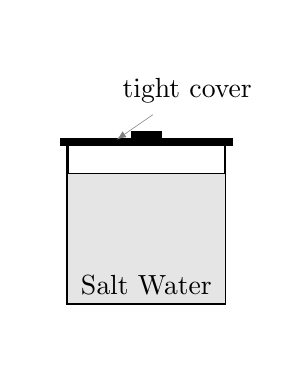
\begin{tikzpicture}
                \draw[white] (-1.5,-0.5) rectangle (1.5,3.5);
                \draw[thick] (-1,2) -- (-1,0) -- (1,0) -- (1,2);
                \draw[thin,fill=white!90!black] (-1,0) rectangle (1,1.66);
                \node[anchor=south] at (0,0) {Salt Water};
                \fill (-1.1,2.0) rectangle (1.1,2.1);
                \fill (-0.2,2.1) rectangle (0.2,2.2);
                \node[pin={[pin distance=2ex,pin edge={latex-,shorten >=1pt}]80:tight cover}] at (-0.5,2.0) {};
            \end{tikzpicture}
        }
    \end{choices}
    \end{multicols}
\end{question}
}

\element{nysed}{
\begin{question}{June1994-Q75}
    A crystalline solid at a temperature below its melting point is heated at a constant rate to a temperature above its melting point.
    Which graph best represents the average internal kinetic energy (KE\textsubscript{ave}) of the substance as a function of heat added?
    \begin{multicols}{2}
    \begin{choices}
        \AMCboxDimensions{down=-1cm}
        \wrongchoice{
            \begin{tikzpicture}
                \begin{axis}[
                    axis y line=left,
                    axis x line=bottom,
                    axis line style={->},
                    xlabel={heat added},
                    xtick=\empty,
                    ylabel={KE\textsubscript{ave}},
                    ytick=\empty,
                    xmin=0,xmax=11,
                    ymin=0,ymax=11,
                    width=0.90\columnwidth,
                    clip=false,
                    very thin,
                ]
                \addplot[line width=1pt,domain=0:10] {7};
                \end{axis}
            \end{tikzpicture}
        }
        \wrongchoice{
            \begin{tikzpicture}
                \begin{axis}[
                    axis y line=left,
                    axis x line=bottom,
                    axis line style={->},
                    xlabel={heat added},
                    xtick=\empty,
                    ylabel={KE\textsubscript{ave}},
                    ytick=\empty,
                    xmin=0,xmax=11,
                    ymin=0,ymax=11,
                    width=0.90\columnwidth,
                    clip=false,
                    very thin,
                ]
                \addplot[line width=1pt,domain=0:10] {x};
                \end{axis}
            \end{tikzpicture}
        }
        %% ANS is 3
        \correctchoice{
            \begin{tikzpicture}
                \begin{axis}[
                    axis y line=left,
                    axis x line=bottom,
                    axis line style={->},
                    xlabel={heat added},
                    xtick=\empty,
                    ylabel={KE\textsubscript{ave}},
                    ytick=\empty,
                    xmin=0,xmax=11,
                    ymin=0,ymax=11,
                    width=0.90\columnwidth,
                    clip=false,
                    very thin,
                ]
                \addplot[line width=1pt,mark=\empty] plot coordinates { (0,0) (3,4) (6,4) (9,8)};
                \end{axis}
            \end{tikzpicture}
        }
        \wrongchoice{
            \begin{tikzpicture}
                \begin{axis}[
                    axis y line=left,
                    axis x line=bottom,
                    axis line style={->},
                    xlabel={heat added},
                    xtick=\empty,
                    ylabel={KE\textsubscript{ave}},
                    ytick=\empty,
                    xmin=0,xmax=11,
                    ymin=0,ymax=11,
                    width=0.90\columnwidth,
                    clip=false,
                    very thin,
                ]
                \addplot[line width=1pt,mark=\empty] plot coordinates { (0,4) (4,4) (10,6)};
                \end{axis}
            \end{tikzpicture}
        }
    \end{choices}
    \end{multicols}
\end{question}
}


%% Section June1990
%%--------------------
\element{nysed}{
\begin{question}{June1990-Q71}
    The minimum average kinetic energy of the molecules in a substance occurs at a temperature of
    \begin{multicols}{2}
    \begin{choices}
        \wrongchoice{\SI{-273}{\kelvin}}
        \wrongchoice{\SI{273}{\degreeCelsius}}
        \wrongchoice{\SI{0}{\degreeCelsius}}
      \correctchoice{\SI{0}{\kelvin}}
    \end{choices}
    \end{multicols}
\end{question}
}

\element{nysed}{
\begin{question}{June1990-Q72}
    How much heat is required to raise the temperature of \SI{1.00}{\kilo\gram} of liquid alcohol from its melting point to \SI{0}{\degreeCelsius}?
    \begin{multicols}{2}
    \begin{choices}
        \wrongchoice{\SI{2.43}{\kilo\joule}}
        \wrongchoice{\SI{196}{\kilo\joule}}
      \correctchoice{\SI{284}{\kilo\joule}}
        \wrongchoice{\SI{476}{\kilo\joule}}
    \end{choices}
    \end{multicols}
\end{question}
}

\newcommand{\nysedJuneNineteenNinetyQSeventyThree}{
\begin{tikzpicture}
    \begin{axis}[
        axis y line=left,
        axis x line=bottom,
        axis line style={->},
        xlabel={time},
        x unit=\si{\minute},
        xtick={0,4,8,12,16,20,24,28,32,36},
        minor x tick num=1,
        ylabel={temperature},
        y unit=\si{\degreeCelsius},
        ytick={0,40,80,120,160,200},
        minor y tick num=1,
        grid=major,
        xmin=0,xmax=36,
        ymin=0,ymax=200,
        width=0.8\columnwidth,
        height=0.5\columnwidth,
        very thin,
    ]
    \addplot[line width=1pt,mark=\empty] plot coordinates { (0,200) (6,140) (14,140) (30,60) (34,60) (36,20) };
    \end{axis}
\end{tikzpicture}
}

\element{nysed}{
\begin{question}{June1990-Q73}
    The graph below represents the variation in temperature as \SI{1.0}{\kilo\gram} of a gas,
        originally at \SI{200}{\degreeCelsius}, loses heat at a constant rate of \SI{2.0}{\kilo\joule\per\minute} and eventually becomes a solid at room temperature.
    \begin{center}
        \nysedJuneNineteenNinetyQSeventyThree
    \end{center}
    What is the heat of fusion of this substance?
    \begin{multicols}{2}
    \begin{choices}
        \wrongchoice{\SI{18}{\kilo\joule\per\kilo\gram}}
        \wrongchoice{\SI{9}{\kilo\joule\per\kilo\gram}}
      \correctchoice{\SI{8}{\kilo\joule\per\kilo\gram}}
        \wrongchoice{\SI{4}{\kilo\joule\per\kilo\gram}}
    \end{choices}
    \end{multicols}
\end{question}
}

\element{nysed}{
\begin{question}{June1990-Q74}
    The graph below represents the variation in temperature as \SI{1.0}{\kilo\gram} of a gas,
        originally at \SI{200}{\degreeCelsius}, loses heat at a constant rate of \SI{2.0}{\kilo\joule\per\minute} and eventually becomes a solid at room temperature.
    \begin{center}
        \nysedJuneNineteenNinetyQSeventyThree
    \end{center}
    What is the boiling temperature of this substance?
    \begin{multicols}{2}
    \begin{choices}
        \wrongchoice{\SI{200}{\degreeCelsius}}
      \correctchoice{\SI{140}{\degreeCelsius}}
        \wrongchoice{\SI{90}{\degreeCelsius}}
        \wrongchoice{\SI{60}{\degreeCelsius}}
    \end{choices}
    \end{multicols}
\end{question}
}

\element{nysed}{
\begin{question}{June1990-Q75}
    The graph below represents the variation in temperature as \SI{1.0}{\kilo\gram} of a gas,
        originally at \SI{200}{\degreeCelsius}, loses heat at a constant rate of \SI{2.0}{\kilo\joule\per\minute} and eventually becomes a solid at room temperature.
    \begin{center}
        \nysedJuneNineteenNinetyQSeventyThree
    \end{center}
    Which phase has the highest specific heat?
    \begin{multicols}{3}
    \begin{choices}
        \wrongchoice{solid}
      \correctchoice{liquid}
        \wrongchoice{gas}
    \end{choices}
    \end{multicols}
\end{question}
}

\element{nysed}{
\begin{question}{June1990-Q76}
    Which graph best represents the relationship between volume and absolute temperature for an ideal gas at constant pressure?
    \begin{multicols}{2}
    \begin{choices}
        \AMCboxDimensions{down=-2.5em}
        %% ANS is 1
        \correctchoice{
            \begin{tikzpicture}
                \begin{axis}[
                    axis y line=left,
                    axis x line=bottom,
                    axis line style={->},
                    xlabel={temperature},
                    xtick=\empty,
                    ylabel={volume},
                    ytick=\empty,
                    xmin=0,xmax=11,
                    ymin=0,ymax=11,
                    width=\columnwidth,
                    very thin,
                ]
                \addplot[line width=1pt,domain=0:10]{x};
                \end{axis}
            \end{tikzpicture}
        }
        \wrongchoice{
            \begin{tikzpicture}
                \begin{axis}[
                    axis y line=left,
                    axis x line=bottom,
                    axis line style={->},
                    xlabel={temperature},
                    xtick=\empty,
                    ylabel={volume},
                    ytick=\empty,
                    xmin=0,xmax=11,
                    ymin=0,ymax=11,
                    width=\columnwidth,
                    very thin,
                ]
                \addplot[line width=1pt,domain=0:10]{6};
                \end{axis}
            \end{tikzpicture}
        }
        \wrongchoice{
            \begin{tikzpicture}
                \begin{axis}[
                    axis y line=left,
                    axis x line=bottom,
                    axis line style={->},
                    xlabel={temperature},
                    xtick=\empty,
                    ylabel={volume},
                    ytick=\empty,
                    xmin=0,xmax=11,
                    ymin=0,ymax=11,
                    width=\columnwidth,
                    very thin,
                ]
                %% changed function
                \addplot[line width=1pt,domain=0:10]{0.1*x*x};
                \end{axis}
            \end{tikzpicture}
        }
        \wrongchoice{
            \begin{tikzpicture}
                \begin{axis}[
                    axis y line=left,
                    axis x line=bottom,
                    axis line style={->},
                    xlabel={temperature},
                    xtick=\empty,
                    ylabel={volume},
                    ytick=\empty,
                    xmin=0,xmax=11,
                    ymin=0,ymax=11,
                    width=\columnwidth,
                    very thin,
                ]
                \addplot[line width=1pt,domain=0:10]{10/x};
                \end{axis}
            \end{tikzpicture}
        }
    \end{choices}
    \end{multicols}
\end{question}
}

\element{nysed}{
\begin{question}{June1990-Q77}
    In an ideal gas, entropy is a measure of the:
    \begin{choices}
        \wrongchoice{volume of the molecules}
        \wrongchoice{mass of the molecules}
        \wrongchoice{forces of attraction between the molecules}
      \correctchoice{disorder of the molecules}
    \end{choices}
\end{question}
}

\element{nysed}{
\begin{question}{June1990-Q78}
    As the pressure of a fixed mass of gas is increased at constant temperature,
        the density of that gas:
    \begin{choices}
        \wrongchoice{decreases}
      \correctchoice{increases}
        \wrongchoice{remains the same}
    \end{choices}
\end{question}
}

\element{nysed}{
\begin{question}{June1990-Q79}
    After a hot object is placed in an insulated container with a cold object,
        the hot object changes temperature and the cold object changes phase.
    The total amount of internal energy in the system will
    \begin{choices}
        \wrongchoice{decreases}
        \wrongchoice{increases}
      \correctchoice{remains the same}
    \end{choices}
\end{question}
}

\element{nysed}{
\begin{question}{June1990-Q80}
    Compared to the freezing point of pure water,
        the freezing point of a salt-water solution is:
    \begin{multicols}{3}
    \begin{choices}
      \correctchoice{lower}
        \wrongchoice{highers}
        \wrongchoice{the same}
    \end{choices}
    \end{multicols}
\end{question}
}


%% Section June1989
%%--------------------
\element{nysed}{
\begin{question}{June1989-Q71}
    A temperature change of \SI{51}{\degreeCelsius} would be equivalent to a temperature change of:
    \begin{multicols}{2}
    \begin{choices}
      \correctchoice{\SI{51}{\kelvin}}
        \wrongchoice{\SI{324}{\kelvin}}
        \wrongchoice{\SI{222}{\kelvin}}
        \wrongchoice{\SI{-222}{\kelvin}}
    \end{choices}
    \end{multicols}
\end{question}
}

\element{nysed}{
\begin{question}{June1989-Q72}
    For object $A$ to have a higher absolute temperature than object $B$,
        object $A$ must have a:
    \begin{choices}
        \wrongchoice{higher average internal potential energy}
      \correctchoice{higher average internal kinetic energy}
        \wrongchoice{greater mass}
        \wrongchoice{greater specific heat}
    \end{choices}
\end{question}
}

\element{nysed}{
\begin{question}{June1989-Q73}
    The graph below represents the relationship between the temperature of a gas and the average kinetic energy (KE) of the molecules of the gas.
    \begin{center}
    \begin{tikzpicture}
        \begin{axis}[
            axis y line=middle,
            axis x line=bottom,
            axis line style={->},
            xlabel={temperature},
            xtick=\empty,
            ylabel={kinetic energy},
            ytick=\empty,
            y label style={
                at={(current axis.above origin)},
                anchor=south east,
                rotate=90,
            },
            xmin=-300,xmax=300,
            ymin=0,ymax=150,
            width=1.0\columnwidth,
            height=0.618\columnwidth,
            clip=false,
            very thin,
        ]
        \addplot[line width=1pt,domain=-273:300]{0.2*(x+273)};
        \fill (axis cs:-273,0) circle (2pt) node[anchor=north] {$X$};
        \end{axis}
    \end{tikzpicture}
    \end{center}
    The temperature represented at point $X$ is approximately:
    \begin{multicols}{2}
    \begin{choices}
        \wrongchoice{\SI{273}{\degreeCelsius}}
        \wrongchoice{\SI{0}{\degreeCelsius}}
      \correctchoice{\SI{-273}{\degreeCelsius}}
        \wrongchoice{\SI{-373}{\degreeCelsius}}
    \end{choices}
    \end{multicols}
\end{question}
}

\element{nysed}{
\begin{question}{June1989-Q74}
    If \SI{73}{\kilo\joule} of heat energy is added to \SI{1.50}{\kilo\gram} of ethyl alcohol initially at \SI{20}{\degreeCelsius},
        what will be the final temperature of the liquid?
    \begin{multicols}{2}
    \begin{choices}
        \wrongchoice{\SI{20}{\degreeCelsius}}
        \wrongchoice{\SI{22}{\degreeCelsius}}
      \correctchoice{\SI{40}{\degreeCelsius}}
        \wrongchoice{\SI{60}{\degreeCelsius}}
    \end{choices}
    \end{multicols}
\end{question}
}

\element{nysed}{
\begin{question}{June1989-Q75}
    Equal masses of copper, iron, lead, and silver are heated from \SI{20}{\degreeCelsius} to \SI{100}{\degreeCelsius}.
    Which substance absorbs the \emph{least} amount of heat?
    \begin{multicols}{2}
    \begin{choices}
      \correctchoice{lead}
        \wrongchoice{iron}
        \wrongchoice{copper}
        \wrongchoice{silver}
    \end{choices}
    \end{multicols}
\end{question}
}

\element{nysed}{
\begin{question}{June1989-Q76}
    Block $A$, at \SI{100}{\degreeCelsius}, and block $B$, at \SI{50}{\degreeCelsius},
        are brought together in a well-insulated container.
    The internal energy of block $A$ will:
    \begin{choices}
        \wrongchoice{decrease and the internal energy of block $B$ will decrease.}
      \correctchoice{decrease and the internal energy of block $B$ will increase.}
        \wrongchoice{increase and the internal energy of block $B$ will decrease.}
        \wrongchoice{increase and the internal energy of block $B$ will increase.}
    \end{choices}
\end{question}
}

\element{nysed}{
\begin{question}{June1989-Q77}
    Which graph best represents the relationship between the heat absorbed ($Q$) by a solid and its temperature ($T$)?
    [Assume the specific heat of the solid to be constant.]
    \begin{multicols}{2}
    \begin{choices}
        \AMCboxDimensions{down=-2.5em}
        \wrongchoice{
            \begin{tikzpicture}
                \begin{axis}[
                    axis y line=left,
                    axis x line=bottom,
                    axis line style={->},
                    xlabel={heat},
                    y unit=\si{\joule},
                    xtick=\empty,
                    ylabel={temperature},
                    y unit=\si{\degreeCelsius},
                    ytick=\empty,
                    xmin=0,xmax=11,
                    ymin=0,ymax=11,
                    width=\columnwidth,
                    very thin,
                ]
                \addplot[line width=1pt,domain=0:10]{0.1*x*x};
                \end{axis}
            \end{tikzpicture}
        }
        \wrongchoice{
            \begin{tikzpicture}
                \begin{axis}[
                    axis y line=left,
                    axis x line=bottom,
                    axis line style={->},
                    xlabel={heat},
                    y unit=\si{\joule},
                    xtick=\empty,
                    ylabel={temperature},
                    y unit=\si{\degreeCelsius},
                    ytick=\empty,
                    xmin=0,xmax=11,
                    ymin=0,ymax=11,
                    width=\columnwidth,
                    very thin,
                ]
                \addplot[line width=1pt,domain=0:10]{sqrt(10)*sqrt(x)};
                \end{axis}
            \end{tikzpicture}
        }
        \wrongchoice{
            \begin{tikzpicture}
                \begin{axis}[
                    axis y line=left,
                    axis x line=bottom,
                    axis line style={->},
                    xlabel={heat},
                    y unit=\si{\joule},
                    xtick=\empty,
                    ylabel={temperature},
                    y unit=\si{\degreeCelsius},
                    ytick=\empty,
                    xmin=0,xmax=11,
                    ymin=0,ymax=11,
                    width=\columnwidth,
                    very thin,
                ]
                \addplot[line width=1pt,domain=0:10]{6};
                \end{axis}
            \end{tikzpicture}
        }
        %% ANS is 4
        \correctchoice{
            \begin{tikzpicture}
                \begin{axis}[
                    axis y line=left,
                    axis x line=bottom,
                    axis line style={->},
                    xlabel={heat},
                    y unit=\si{\joule},
                    xtick=\empty,
                    ylabel={temperature},
                    y unit=\si{\degreeCelsius},
                    ytick=\empty,
                    xmin=0,xmax=11,
                    ymin=0,ymax=11,
                    width=\columnwidth,
                    very thin,
                ]
                \addplot[line width=1pt,domain=0:10]{x};
                \end{axis}
            \end{tikzpicture}
        }
    \end{choices}
    \end{multicols}
\end{question}
}

\element{nysed}{
\begin{question}{June1989-Q78}
    A given mass of gas is enclosed in a rigid container.
    If the velocity of the gas molecules colliding with the sides of the container increases,
        the:
    \begin{choices}
        \wrongchoice{density of the gas will increase.}
      \correctchoice{pressure of the gas will increase.}
        \wrongchoice{density of the gas will decrease.}
        \wrongchoice{pressure of the gas will decrease.}
    \end{choices}
\end{question}
}

\element{nysed}{
\begin{question}{June1989-Q79}
    The absolute temperature of a fixed mass of ideal gas is tripled while its volume remains constant.
    The ratio of the final pressure of the gas to its initial pressure is:
    \begin{multicols}{2}
    \begin{choices}
        \wrongchoice{1 to 1}
        \wrongchoice{1.5 to 1}
      \correctchoice{3 to 1}
        \wrongchoice{9 to 1}
    \end{choices}
    \end{multicols}
\end{question}
}

\element{nysed}{
\begin{question}{June1989-Q80}
    Compared to the boiling point of pure water,
        the boiling point of a salt-water solution is:
    \begin{multicols}{3}
    \begin{choices}
        \wrongchoice{lower}
      \correctchoice{higher}
        \wrongchoice{the same}
    \end{choices}
    \end{multicols}
\end{question}
}


%% Section June1986
%%--------------------
\element{nysed}{
\begin{question}{June1986-Q18}
    Which quantity is the equivalent to \SI{840}{\joule}?
    \begin{multicols}{2}
    \begin{choices}
      \correctchoice{\SI{0.20}{\kilo\calorie}}
        \wrongchoice{\SI{8.4}{\kilo\calorie}}
        \wrongchoice{\SI{42}{\kilo\calorie}}
        \wrongchoice{\SI{64}{\kilo\calorie}}
    \end{choices}
    \end{multicols}
\end{question}
}

\element{nysed}{
\begin{question}{June1986-Q20}
    Which graph best represents the relationship between the absolute temperature ($T_K$) of an ideal gas and the average kinetic energy ($\bar{E}_k$) of its molecules?
    \begin{multicols}{2}
    \begin{choices}
        \AMCboxDimensions{down=-2.5em}
        \wrongchoice{
            \begin{tikzpicture}
                \begin{axis}[
                    axis y line=left,
                    axis x line=bottom,
                    axis line style={->},
                    xlabel={$T_k$},
                    xtick=\empty,
                    ylabel={$\bar{E}_k$},
                    ytick=\empty,
                    xmin=0,xmax=11,
                    ymin=0,ymax=11,
                    width=\columnwidth,
                    very thin,
                ]
                \addplot[line width=1pt,domain=0:10]{10-x};
                \end{axis}
            \end{tikzpicture}
        }
        \wrongchoice{
            \begin{tikzpicture}
                \begin{axis}[
                    axis y line=left,
                    axis x line=bottom,
                    axis line style={->},
                    xlabel={$T_k$},
                    xtick=\empty,
                    ylabel={$\bar{E}_k$},
                    ytick=\empty,
                    xmin=0,xmax=11,
                    ymin=0,ymax=11,
                    width=\columnwidth,
                    very thin,
                ]
                \addplot[line width=1pt,domain=0:10]{10/x};
                \end{axis}
            \end{tikzpicture}
        }
        \wrongchoice{
            \begin{tikzpicture}
                \begin{axis}[
                    axis y line=left,
                    axis x line=bottom,
                    axis line style={->},
                    xlabel={$T_k$},
                    xtick=\empty,
                    ylabel={$\bar{E}_k$},
                    ytick=\empty,
                    xmin=0,xmax=11,
                    ymin=0,ymax=11,
                    width=\columnwidth,
                    very thin,
                ]
                \addplot[line width=1pt,domain=0:10]{0.1*x*x};
                \end{axis}
            \end{tikzpicture}
        }
        %% ANS is 4
        \correctchoice{
            \begin{tikzpicture}
                \begin{axis}[
                    axis y line=left,
                    axis x line=bottom,
                    axis line style={->},
                    xlabel={$T_k$},
                    xtick=\empty,
                    ylabel={$\bar{E}_k$},
                    ytick=\empty,
                    xmin=0,xmax=11,
                    ymin=0,ymax=11,
                    width=\columnwidth,
                    very thin,
                ]
                \addplot[line width=1pt,domain=0:10]{x};
                \end{axis}
            \end{tikzpicture}
        }
    \end{choices}
    \end{multicols}
\end{question}
}

\element{nysed}{
\begin{question}{June1986-Q21}
    What is the normal melting point of lead?
    \begin{multicols}{2}
    \begin{choices}
        \wrongchoice{\SI{600}{\degreeCelsius}}
      \correctchoice{\SI{327}{\degreeCelsius}}
        \wrongchoice{\SI{273}{\degreeCelsius}}
        \wrongchoice{\SI{0}{\degreeCelsius}}
    \end{choices}
    \end{multicols}
\end{question}
}

\element{nysed}{
\begin{question}{June1986-Q66}
    A \SI{0.20}{\kilo\gram} sample of lead at \SI{120}{\degreeCelsius} is put into a calorimeter containing \SI{0.30}{\kilo\gram} of water at \SI{18}{\degreeCelsius}.
    The equilibrium temperature of the mixture is \SI{20}{\degreeCelsius}.
    [Assume that the calorimeter does not absorb heat.]
    %% start question
    How much heat is lost by the lead sample?
    \begin{multicols}{2}
    \begin{choices}
      \correctchoice{\SI{0.60}{\kilo\calorie}}
        \wrongchoice{\SI{20}{\kilo\calorie}}
        \wrongchoice{\SI{3.0}{\kilo\calorie}}
        \wrongchoice{\SI{100}{\kilo\calorie}}
    \end{choices}
    \end{multicols}
\end{question}
}

\element{nysed}{
\begin{question}{June1986-Q67}
    A \SI{0.20}{\kilo\gram} sample of lead at \SI{120}{\degreeCelsius} is put into a calorimeter containing \SI{0.30}{\kilo\gram} of water at \SI{18}{\degreeCelsius}.
    The equilibrium temperature of the mixture is \SI{20}{\degreeCelsius}.
    [Assume that the calorimeter does not absorb heat.]
    %% start question
    Compared to the heat lost by the lead,
        the heat gained by the water is:
    \begin{multicols}{3}
    \begin{choices}
        \wrongchoice{less}
        \wrongchoice{more}
      \correctchoice{the same}
    \end{choices}
    \end{multicols}
\end{question}
}

\element{nysed}{
\begin{question}{June1986-Q68}
    A \SI{0.20}{\kilo\gram} sample of lead at \SI{120}{\degreeCelsius} is put into a calorimeter containing \SI{0.30}{\kilo\gram} of water at \SI{18}{\degreeCelsius}.
    The equilibrium temperature of the mixture is \SI{20}{\degreeCelsius}.
    [Assume that the calorimeter does not absorb heat.]
    %% start question
    The problem above is repeated using \SI{0.20}{\kilo\gram} of zinc instead of lead.
    All other initial conditions remain the same.
    Compared to the water temperature change when lead was used,
        the water temperature change when zinc is used is:
    \begin{multicols}{3}
    \begin{choices}
        \wrongchoice{smaller}
      \correctchoice{larger}
        \wrongchoice{the same}
    \end{choices}
    \end{multicols}
\end{question}
}


%% Section June1985
%%--------------------
\element{nysed}{
\begin{question}{June1985-Q16}
    A change in the average kinetic energy of the molecules of an object may best be detected by measuring a change in the object's:
    \begin{multicols}{2}
    \begin{choices}
        \wrongchoice{mass}
        \wrongchoice{speed}
        \wrongchoice{weight}
      \correctchoice{temperature}
    \end{choices}
    \end{multicols}
\end{question}
}

\element{nysed}{
\begin{question}{June1985-Q17}
    Which graph best represents the relationship between the Kelvin temperature scale the degree Celsius temperature scale?
    \begin{multicols}{2}
    \begin{choices}
        \AMCboxDimensions{down=-2.5em}
        \wrongchoice{
            \begin{tikzpicture}
                \begin{axis}[
                    axis y line=left,
                    axis x line=bottom,
                    axis line style={->},
                    xlabel={Celsius},
                    x label style={
                        at={(current axis.right of origin)},
                        anchor=north east,
                    },
                    xtick=\empty,
                    ylabel={kelvin},
                    y label style={
                        at={(current axis.above origin)},
                        anchor=south east,
                    },
                    ytick=\empty,
                    xmin=0,xmax=11,
                    ymin=0,ymax=11,
                    width=\columnwidth,
                    very thin,
                ]
                \addplot[line width=1pt,domain=0:10]{x};
                \end{axis}
            \end{tikzpicture}
        }
        %% ANS is 2
        \correctchoice{
            \begin{tikzpicture}
                \begin{axis}[
                    axis y line=left,
                    axis x line=bottom,
                    axis line style={->},
                    xlabel={Celsius},
                    x label style={
                        at={(current axis.right of origin)},
                        anchor=north east,
                    },
                    xtick=\empty,
                    ylabel={kelvin},
                    ytick={2},
                    %% corrected error
                    yticklabels={\num{273}},
                    y tick label style={rotate=90,anchor=south},
                    y label style={
                        at={(current axis.above origin)},
                        anchor=south east,
                    },
                    xmin=0,xmax=11,
                    ymin=0,ymax=11,
                    width=\columnwidth,
                    very thin,
                ]
                \addplot[line width=1pt,domain=0:8]{0.9*x+2};
                \end{axis}
            \end{tikzpicture}
        }
        \wrongchoice{
            \begin{tikzpicture}
                \begin{axis}[
                    axis y line=left,
                    axis x line=bottom,
                    axis line style={->},
                    xlabel={Celsius},
                    x label style={
                        at={(current axis.right of origin)},
                        anchor=north east,
                    },
                    xtick=\empty,
                    ylabel={kelvin},
                    y label style={
                        at={(current axis.above origin)},
                        anchor=south east,
                    },
                    ytick=\empty,
                    xmin=0,xmax=11,
                    ymin=0,ymax=11,
                    width=\columnwidth,
                    very thin,
                ]
                \addplot[line width=1pt,domain=0:10]{1+0.09*x*x};
                \end{axis}
            \end{tikzpicture}
        }
        \wrongchoice{
            \begin{tikzpicture}
                \begin{axis}[
                    axis y line=left,
                    axis x line=bottom,
                    axis line style={->},
                    xlabel={Celsius},
                    x label style={
                        at={(current axis.right of origin)},
                        anchor=north east,
                    },
                    xtick={2},
                    xticklabels={\ang{273}},
                    ylabel={kelvin},
                    y label style={
                        at={(current axis.above origin)},
                        anchor=south east,
                    },
                    ytick=\empty,
                    xmin=0,xmax=11,
                    ymin=0,ymax=11,
                    width=\columnwidth,
                    very thin,
                ]
                \addplot[line width=1pt,domain=2:10]{x-2};
                \end{axis}
            \end{tikzpicture}
        }
    \end{choices}
    \end{multicols}
\end{question}
}

\newcommand{\nysedJuneNineteenEightyFiveQSeventyOne}{
\begin{tikzpicture}
    \begin{axis}[
        axis y line=left,
        axis x line=middle,
        axis line style={->},
        xlabel={heat},
        x unit=\si{\kilo\calorie},
        xtick={0,20,40,60,80,100,120},
        minor x tick num=1,
        ylabel={temperature},
        y unit=\si{\degreeCelsius},
        ytick={40,60,80,100},
        minor y tick num=3,
        xmin=0,xmax=120,
        ymin=40,ymax=100,
        width=0.95\columnwidth,
        height=0.6\columnwidth,
        grid=major,
        clip=false,
        very thin,
    ]
    \addplot[line width=1pt,mark=\empty] plot coordinates {(0,40) (10,60) (30,60) (50,80) (100,80) (120,90)};
    %% phase labels
    \node[anchor=north west] at (axis cs:5,50) {solid};
    \node[anchor=south east] at (axis cs:40,70) {liquid};
    \node[anchor=south east] at (axis cs:110,85) {gas};
    %% letter labels
    \fill (axis cs:0,40) circle (1.5pt) node[anchor=north] {$A$};
    \fill (axis cs:10,60) circle (1.5pt) node[anchor=north west] {$B$};
    \fill (axis cs:30,60) circle (1.5pt) node[anchor=north] {$C$};
    \fill (axis cs:50,80) circle (1.5pt) node[anchor=north west] {$D$};
    \fill (axis cs:100,80) circle (1.5pt) node[anchor=north] {$E$};
    \fill (axis cs:120,90) circle (1.5pt) node[anchor=north] {$F$};
    \end{axis}
\end{tikzpicture}
}

\element{nysed}{
\begin{question}{June1985-Q71}
    The graph below which represents the temperature of \SI{1}{\kilo\gram} of an unidentified substance as heat is added.
    \begin{center}
        \nysedJuneNineteenEightyFiveQSeventyOne
    \end{center}
    What is the boiling point of the substance?
    \begin{multicols}{2}
    \begin{choices}
        \wrongchoice{\SI{40}{\degreeCelsius}}
        \wrongchoice{\SI{60}{\degreeCelsius}}
      \correctchoice{\SI{80}{\degreeCelsius}}
        \wrongchoice{\SI{90}{\degreeCelsius}}
    \end{choices}
    \end{multicols}
\end{question}
}

\element{nysed}{
\begin{question}{June1985-Q72}
    The graph below which represents the temperature of \SI{1}{\kilo\gram} of an unidentified substance as heat is added.
    \begin{center}
        \nysedJuneNineteenEightyFiveQSeventyOne
    \end{center}
    What is the heat of fusion of the substance?
    \begin{multicols}{2}
    \begin{choices}
        \wrongchoice{\SI{10}{\kilo\calorie\per\kilo\gram}}
      \correctchoice{\SI{20}{\kilo\calorie\per\kilo\gram}}
        \wrongchoice{\SI{30}{\kilo\calorie\per\kilo\gram}}
        \wrongchoice{\SI{50}{\kilo\calorie\per\kilo\gram}}
    \end{choices}
    \end{multicols}
\end{question}
}

\element{nysed}{
\begin{question}{June1985-Q73}
    The graph below which represents the temperature of \SI{1}{\kilo\gram} of an unidentified substance as heat is added.
    \begin{center}
        \nysedJuneNineteenEightyFiveQSeventyOne
    \end{center}
    During which interval does the average kinetic energy of the molecules of the substance remain constant?
    \begin{multicols}{4}
    \begin{choices}
        \wrongchoice{$AB$}
        \wrongchoice{$EF$}
        \wrongchoice{$CD$}
      \correctchoice{$DE$}
    \end{choices}
    \end{multicols}
\end{question}
}

\element{nysed}{
\begin{question}{June1985-Q74}
    The graph below which represents the temperature of \SI{1}{\kilo\gram} of an unidentified substance as heat is added.
    \begin{center}
        \nysedJuneNineteenEightyFiveQSeventyOne
    \end{center}
    During which interval is the specific heat of the substance greatest?
    \begin{multicols}{4}
    \begin{choices}
        \wrongchoice{$AB$}
      \correctchoice{$EF$}
        \wrongchoice{$CD$}
        \wrongchoice{$DE$}
    \end{choices}
    \end{multicols}
\end{question}
}

\element{nysed}{
\begin{question}{June1985-Q75}
    The graph below which represents the temperature of \SI{1}{\kilo\gram} of an unidentified substance as heat is added.
    \begin{center}
        \nysedJuneNineteenEightyFiveQSeventyOne
    \end{center}
    As the temperature of a constant volume of an ideal gas is increased,
        its pressure will:
    \begin{choices}
        \wrongchoice{decrease}
      \correctchoice{increase}
        \wrongchoice{remain the same}
    \end{choices}
\end{question}
}


\endinput


